% ---- ETD Document Class and Useful Packages ---- %
\documentclass{ucetd}  % bib file is coded in this
\usepackage{graphicx}
\usepackage{subcaption}
\usepackage{natbib}
\usepackage{amsmath}
\usepackage{amsthm}
\usepackage{amsfonts}
\usepackage{multirow}
\usepackage{microtype}
\usepackage{amssymb}
\usepackage{amsthm}
\usepackage{docmute}
\usepackage{morefloats}
\usepackage{rotating}
\usepackage{wrapfig}
\usepackage{setspace}
\usepackage{parskip}
%\usepackage[nottoc,numbib]{tocbibind}

\newenvironment{section_abstract}{\rightskip1in}{}



%% Use these commands to set biographic information for the title page:
\title{Thesis Title}
\author{Peter David Smits}
\department{Committee on Evolutionary Biology}
\division{Biological Sciences Division}
\degree{Ph.D.}
\date{Graduation Date}

%% Use these commands to set a dedication and epigraph text
\dedication{Dedication Text}
\epigraph{Epigraph Text}



\begin{document}
%% Basic setup commands
% If you don't want a title page comment out the next line and uncomment the line after it:
\maketitle
%\omittitle

% These lines can be commented out to disable the copyright/dedication/epigraph pages
\makecopyright
\makededication
\makeepigraph


%% Make the various tables of contents
\tableofcontents
\listoffigures
\listoftables

\acknowledgments
% Enter Acknowledgements here

\abstract
% Enter Abstract here

\mainmatter
% Main body of text follows

\chapter{Introduction}
% Introductory stuff

% chapter 1
\chapter{Expected time-invariant differences in mammal species duration} \label{ch:death_taxa}

\begin{section_abstract}
 Determining which biological traits influence differences in extinction risk is vital for understanding the differential diversification of life and for making predictions about species' vulnerability to anthropogenic impacts. Here I present a hierarchical Bayesian survival model of North American Cenozoic mammal species durations in relation to species-level ecological factors, time of origination, and phylogenetic relationships. I find support for the ``survival of the unspecialized'' as a time-invariant generalization of trait-based extinction risk. Furthermore, I find that phylogenetic and temporal effects are both substantial factors associated with differences in species durations. Finally, I find that the estimated effects of these factors are partially incongruous with how these factors are correlated with extinction risk of the extant species. This parallels previous observations that background extinction is a poor predictor of mass extinction events and suggests that attention should be focused on mass extinctions to gain insight into modern species loss.
\end{section_abstract}


\section{Introduction}
Why extinction risk varies among species remains one of the most fundamental questions in paleobiology and conservation biology \cite{Simpson1944,VanValen1973,Raup1994,Quental2013,Wagner2014b}. To address this issue, I test for similarities in associations between extinction risk and multiple species-level traits during times of background extinction and in the modern world; which traits have time-invariant effects on species duration; and whether extinction is age-independent. I approach these questions together by using a model of species duration whose parameter estimates act as direct tests of these questions. Cenozoic mammals are an ideal focus for this study because their fossil record is well sampled and well resolved both temporally and spatially, and because individual species ecology and taxonomic position are generally understood \cite{Simpson1944,Quental2013,Alroy2009,Liow2008,Smith2004,Tomiya2013,Marcot2014}. 

Time-invariant factors are those that have a constant directional effect even if their magnitude varies. Because change in the magnitude of extinction risk is not necessarily the best indicator of a shift from background to mass extinction \cite{Wang2003}, it is better to look for changes in either the direction of selection, the loss of a selective pressure, or the appearance of novel selective pressures \cite{Jablonski1986}.

The species-level traits studied here are bioprovince occupancy, body mass, and dietary and locomotor categories. These traits are related to aspects of a species' adaptive zone such as population density, expected range size, potential prey, and dispersal ability \cite{Smith2004,Jernvall2004} and are a combination of aggregate and emergent traits \cite{Jablonski2008a}. It is expected that species with larger geographic ranges have lower extinction rates than species with smaller geographic ranges \cite{Jablonski1986,Roy2009c}; however, how traits more directly related to species--environment interactions may affect species extinction risk is more nebulous.

Body size is a complex trait related to many life history characteristics. There are three general hypotheses of how body size may effect extinction risk: 1) positive effect where an increase in body size causes an increase in extinction risk, potentially due to associated decrease in reproductive rate or other similar life history traits \cite{Liow2008,Liow2009}; 2) negative effect where an increase in body size causes a decrease in extinction risk because of an expected positive relationship between body size and geographic range; and 3) no effect of body size on extinction risk \cite{Tomiya2013}. 

The strongest expectation for the effects of dietary category on extinction risk is that omnivores will have the lowest extinction risk of all species. This expectation is based on the long standing ``survival of the unspecialized'' hypothesis where more generalist species (e.g. omnivores) have greater survival than specialist species (e.g. carnivores/herbivores) \cite{Simpson1944,Liow2004a}. It has also been observed that both carnivores and herbivores have greater diversification rates than omnivores, with herbivores diversifying faster than carnivores \cite{Price2012}. How this result translates into differences in extinction risk is currently unknown \cite{Rabosky2010a}. In modern taxa, higher trophic levels (e.g. carnivores versus herbivores) have been associated with greater extinction risk, most likely because of human extermination of top predators \cite{Liow2009,Purvis2000a}. 

Similarly, there are few expectations of how locomotor category may effect extinction risk. During the Cenozoic, there was a shift at the Paleogene/Neogene boundary from predominately closed to predominately open environments \cite{Blois2009,Janis1993a}. Based on this observation, a prediction is that arboreal taxa will have the greatest extinction risk of all, with both scansorial and ground dwelling taxa having lower extinction risks. 

I use a hierarchical Bayesian survival model of species duration as predicted by the covariates of interest along with species' temporal and phylogenetic context. Species duration, in 2 My bins, was modeled as realizations from either an exponential or Weibull distribution-based hierarchical model \cite{Gelman2013d}. The exponential distribution corresponds to the Law of Constant Extinction, which states that extinction is age-independent \cite{VanValen1973}. Note that the exponential is a special case of the Weibull when its shape parameter, $\alpha$, is 1. The Weibull distribution allows for extinction to be taxon-age dependent, where values of $\alpha$ greater than 1 corresponds to increasing risk with age and values less than 1 corresponds to decreasing risk with age. Origination cohort and phylogenetic position were modeled as independent effects. Phylogenetic effect was modeled assuming species duration may have evolved via a Brownian motion-like process \cite{Lynch1991,Housworth2004}. The results from the Weibull model are detailed here because this model has a better fit to the data the exponential (Weibull WAIC 6140.37, exponential WAIC 16697.35; Fig.~\ref{fig:ppc_surv}, S1, S2).

\begin{figure}[ht]
  \centering
  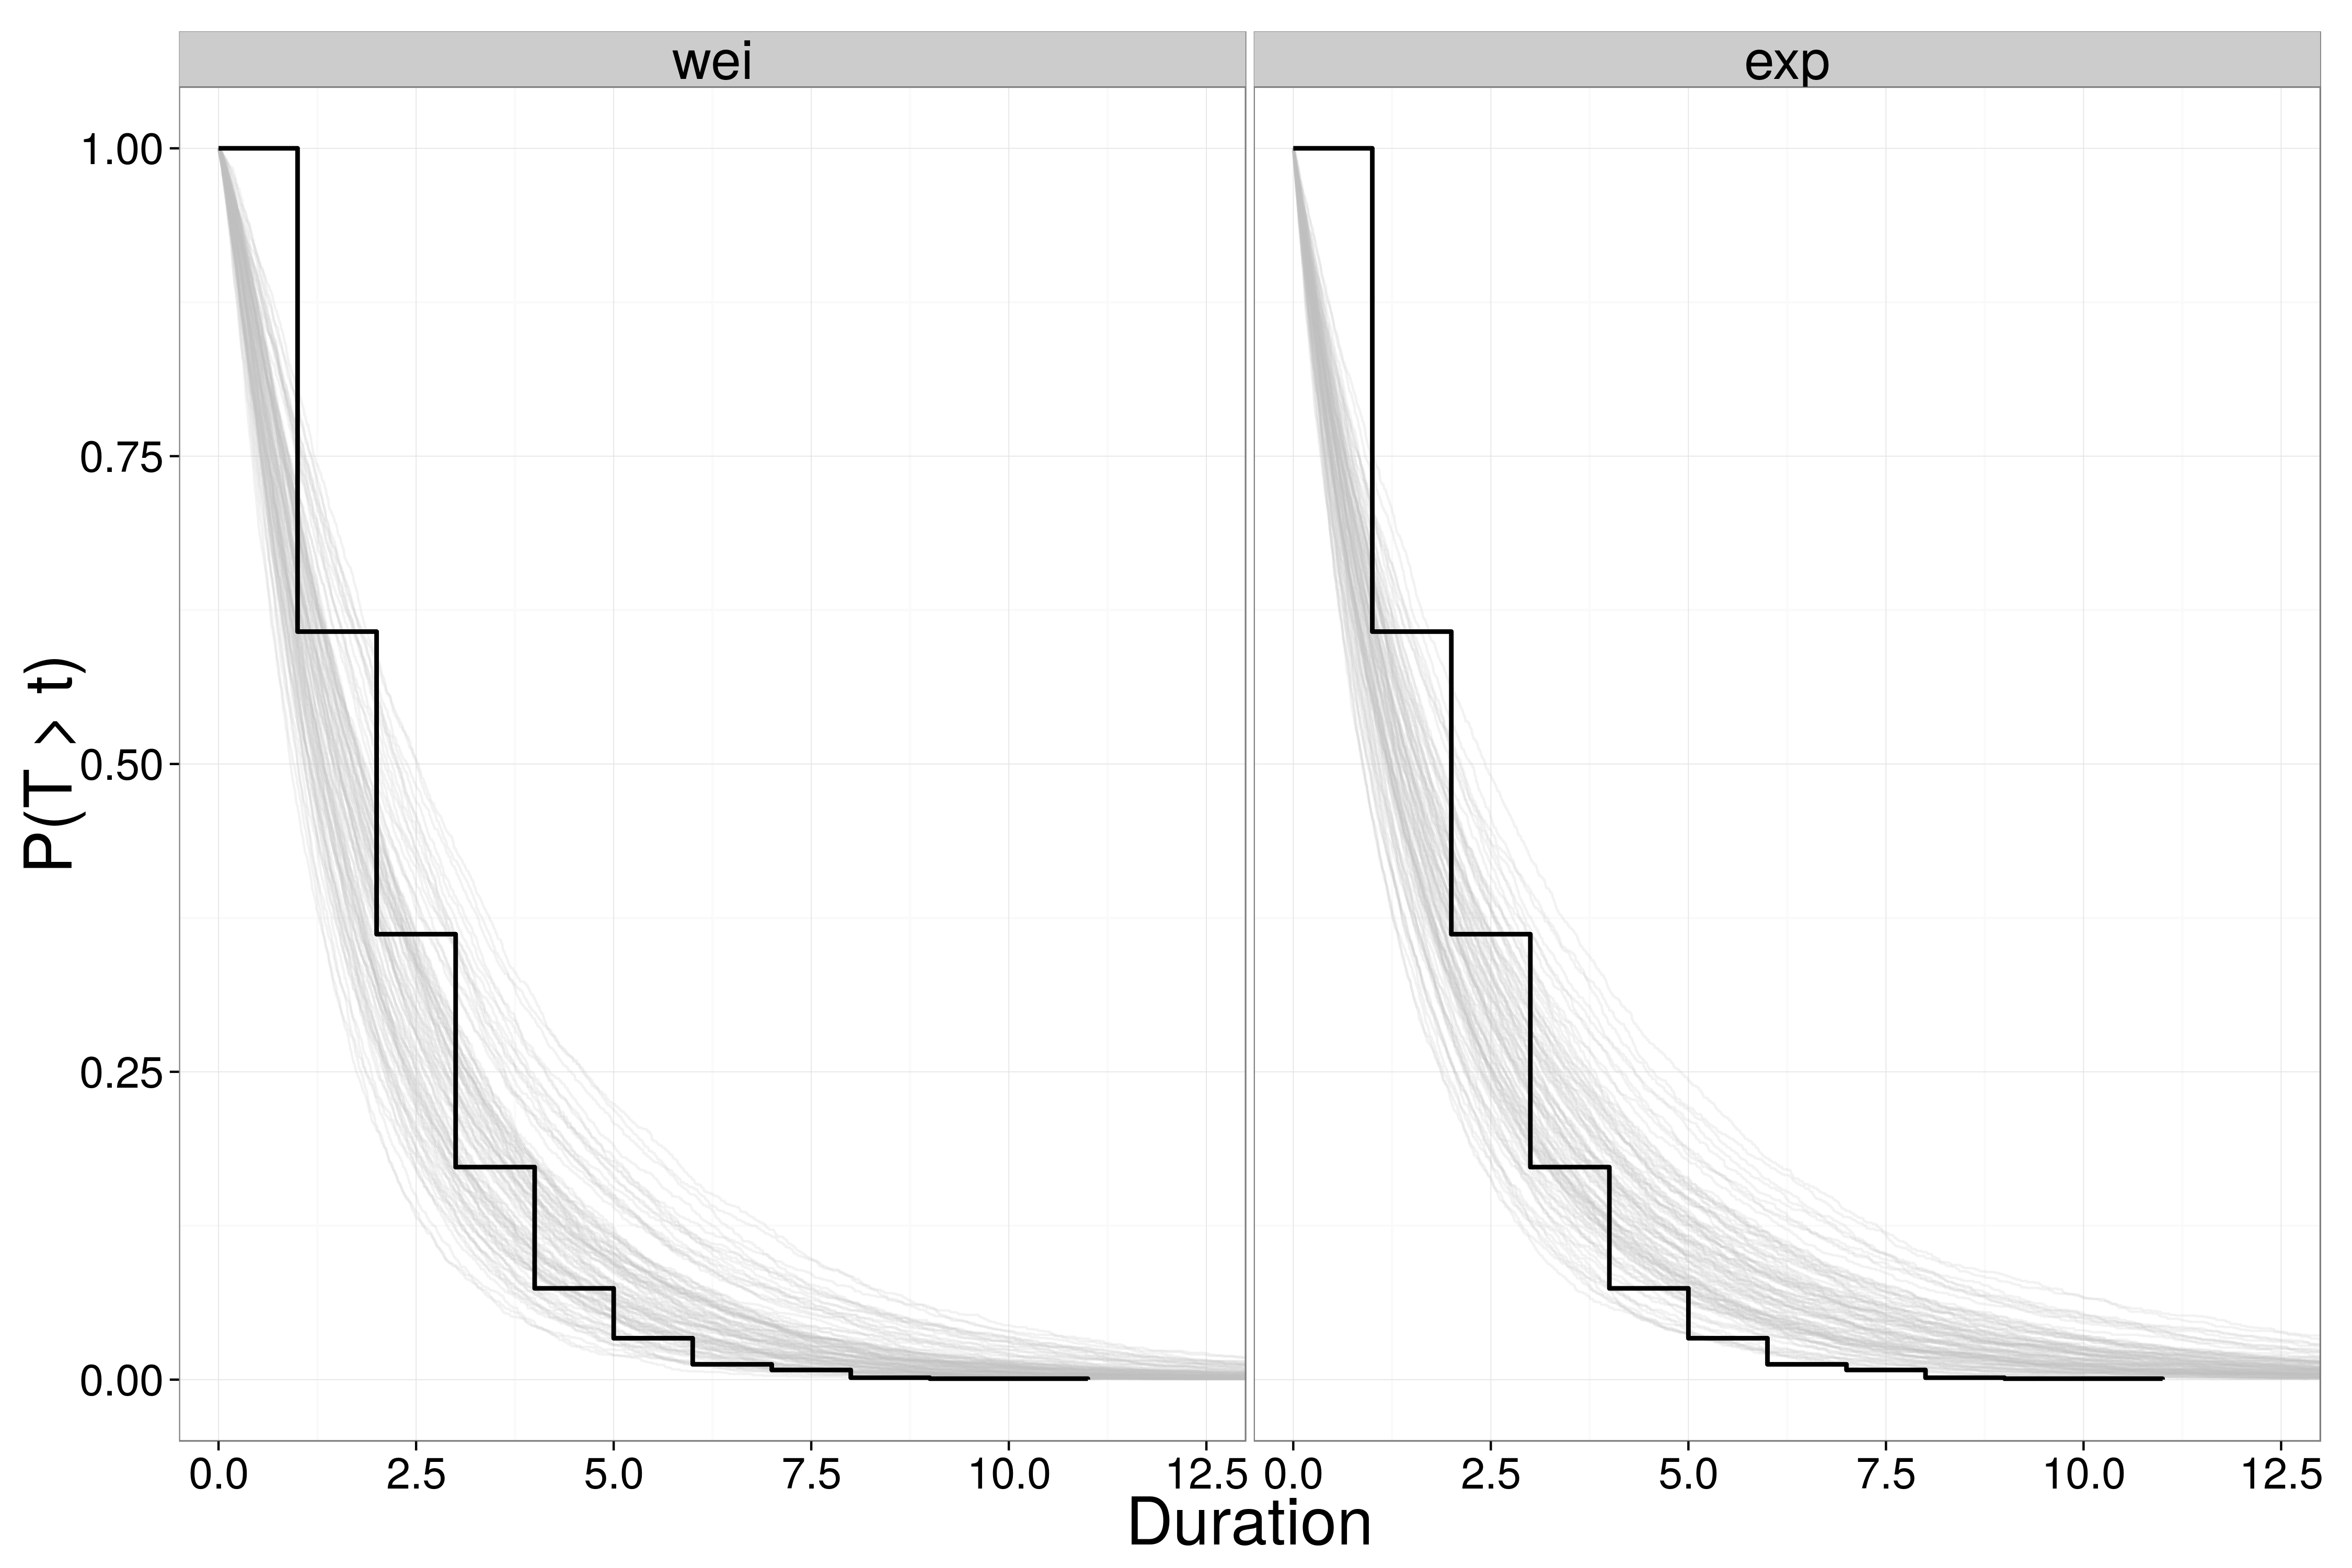
\includegraphics[height=0.3\textheight,width=\textwidth,keepaspectratio=true]{chapter_death_taxa/figure/survival_function}
  \caption[Posterior predictive checks]{Weibull-based model estimates (grey) from 1000 posterior predictive data sets of the empirical survival function (black). The survival function is the probability that a species with duration \(t\) will not have gone extinct. Simulated data sets were generated by drawing parameter values randomly from their estimated posteriors and using the observed covariate information to estimate durations for all the observed species.}
  \label{fig:ppc_surv}
\end{figure}


% show results from exponential model results along side weibull results
%   make sure the signs are the same for exponential and weibull?
%     then I can show estimates together with double histograms?
%     will really help explain the actual results
%   do as two histograms in the same panel for the posterior predictive checks!
%     probably just in supplement
%   results are consistent with which hypotheses?

\section{Results}
\begin{table}[c]
  \centering
  \caption[Posterior estimates of covariates on mammal survival]{Marginal posterior estimates for the praameters of interested based on 1000 posterior samples. The intercept \(\beta_{0}\) can also be interpreted as the estimate for the mean observed species. The remaining \(\beta\) values can be interpreted as the effect of a trait on the expected species duration as expressed as deviation from the mean. The categorical variables are binary index variables where an observation is of that category or not. See Equation \ref{eq:wei_haz} for an explanation of the effect of \(\alpha\) on extinction risk. \(\hat{R}\) values of less than 1.1 indicate approximate chain convergence for the posterior samples.}
  \begin{tabular}{ l l r r r r r r r r }
    parameter & effect & mean & sd & 2.5\% & 25\% & 50\% & 75\% & 97.5\% & \(\hat{R}\) \\ 
    \hline
    \(\alpha\) & ``age'' & 1.29 & 0.03 & 1.23 & 1.27 & 1.29 & 1.31 & 1.36 & 1.00 \\ 
    \hline
    \(\beta_{0}\) & arboreal/carnivore & -0.78 & 0.14 & -1.05 & -0.87 & -0.78 & -0.68 & -0.51 & 1.00 \\ 
    \(\beta_{o}\) & occupancy & -0.53 & 0.08 & -0.69 & -0.59 & -0.53 & -0.48 & -0.38 & 1.00 \\ 
    \(\beta_{size}\) & body size & -0.05 & 0.05 & -0.14 & -0.08 & -0.05 & -0.01 & 0.05 & 1.00 \\ 
    \(\beta_{g}\) & ground dwelling & -0.28 & 0.10 & -0.47 & -0.34 & -0.28 & -0.21 & -0.09 & 1.00 \\ 
    \(\beta_{s}\) & scansorial & -0.22 & 0.11 & -0.43 & -0.29 & -0.22 & -0.14 & -0.00 & 1.00 \\ 
    \(\beta_{h}\) & herbivore & 0.09 & 0.09 & -0.09 & 0.03 & 0.09 & 0.14 & 0.27 & 1.00 \\ 
    \(\beta_{i}\) & insectivore & 0.10 & 0.11 & -0.11 & 0.03 & 0.10 & 0.17 & 0.31 & 1.00 \\ 
    \(\beta_{o}\) & omnivore & -0.12 & 0.11 & -0.33 & -0.19 & -0.12 & -0.05 & 0.09 & 1.00 \\ 
    \hline
    \(\sigma_{c}\) & sd cohort & 0.33 & 0.06 & 0.23 & 0.29 & 0.33 & 0.37 & 0.48 & 1.00 \\ 
    \(\sigma_{p}\) & sd phylogeny & 0.11 & 0.05 & 0.03 & 0.07 & 0.10 & 0.14 & 0.23 & 1.03 \\ 
    \hline
  \end{tabular}
  \label{tab:post_sum}
\end{table}

A summary of the posterior distributions for the most relevant parameter estimates is presented in Table \ref{tab:post_sum}. All posterior inference is based on these estimates. For the results from the posterior predictive checks and discussion of the estimation of $\alpha$, please see the accompanying Supplemental information (Section \ref{sec:death_taxa_supp}). Additionally, see the Supplemental information for discussion surrounding use of Paleobiology Database and accompanying data quality concerns.

Species with greater bioprovince occupancy are found to be associated with lower extinction risk than taxa with smaller bioprovince occupancy (\(\beta_{occupancy} \text{mean} = -0.53\), std \(= 0.08\)). This is consistent with previous findings. Body size has nearly zero association with expected duration (\(\beta_{size} \text{mean} = -0.05\), std \(= 0.05\)), a similar result to some previous studies \cite{Tomiya2013}. However, previous studies were performed at the generic level and were unable to determine how body size may effect species-level extinction, as the effect of either extinction or speciation cannot be distinguished \cite{Liow2008,Tomiya2013}.

Some clear patterns emerge from the pairwise differences in effect of each dietary category on expected duration (Fig.~\ref{fig:trait_est}). Consistent with expectations from the ``survival of the unspecialized'' hypothesis \cite{Liow2004a,Simpson1944}, omnivory appears to be associated with the lowest expected extinction risk. Carnivory is associated a greater expected duration than either herbivory or insectivory, but a greater expected extinction risk than omnivory. Finally, herbivory and insectivory have approximately equal effects on expected duration. Given previous results, these results imply that carnivores have a greater origination rate than omnivores \cite{Price2012}. These results also imply that herbivores, which have the greatest extinction risk, must also have a very high origination rate in order to have the greatest diversification rate among these three categories \cite{Price2012}. 

\begin{figure}[ht]
  \centering
  \begin{subfigure}[b]{0.45\textwidth}
    \caption{}
    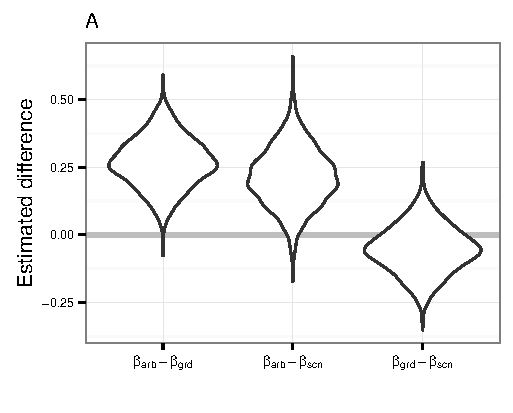
\includegraphics[height=0.3\textheight,width=\textwidth,keepaspectratio=true]{chapter_death_taxa/figure/loco_diff_est}
    \label{subfig:loco}
  \end{subfigure}
  \begin{subfigure}[b]{0.45\textwidth}
    \caption{}
    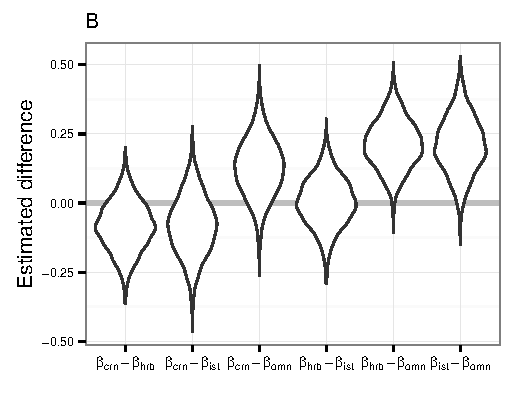
\includegraphics[height=0.3\textheight,width=\textwidth,keepaspectratio=true]{chapter_death_taxa/figure/diet_diff_est}
    \label{subfig:diet}
  \end{subfigure}
  \caption[Effect of mammal ecotypes on survival]{Pairwise differences in effect of the locomotor (\textbf{A}) and dietary categories (\textbf{B}) on expected duration from 1000 samples from the posterior distribution. Comparisons of locomotor categories, from top to bottom (\textbf{A}), are: arboreal (\(\beta_{arb} = \beta_{0}\)) versus ground dwelling (\(\beta_{grd} = \beta_{0} + \beta_{g}\)), arboreal versus scansorial (\(\beta_{scn} = \beta_{0} + \beta_{s}\)), and ground dwelling versus scansorial. For dietary category, from top to bottom (\textbf{B}): carnivore (\(\beta_{crn} = \beta_{0}\)) versus herbivore (\(\beta_{hrb} = \beta_{0} + \beta_{h}\)), carnivore versus insectivore (\(\beta_{ist} = \beta_{0} + \beta_{i}\)), carnivore versus omnivore (\(\beta_{omn} = \beta_{0} + \beta_{o}\)), herbivore versus insectivore, herbivore versus omnivore, and insectivore versus omnivore. Negative values indicate that the first category is expected to have a greater duration than the second, while positive values indicate that the first category is expected to have a shorter duration.}
  \label{fig:trait_est}
\end{figure}

For locomotor category, both scansoriality and ground dwelling life habitat are associated with a greater expected duration than arboreality (Fig.~\ref{fig:trait_est}). Scansorial and ground dwelling life habits also have approximately equal expected effects on extinction risk.  This is consistent with the expectation that arboreality will confer greater extinction risk due to the loss of associated environment with the shift from open to closed habitat at the Paleogene/Neogene boundary \cite{Blois2009}. However, there are two possible processes which could lead to the observed pattern: arboreality confers an intrinsic difference in extinction risk or it might not be that arboreal taxa have an intrinsically higher risk but were instead ``hit harder'' by the environmental shift than other taxa. This analysis cannot distinguish between these two processes. Note that, while this is a study of North American Cenozoic mammals, for European Cenozoic mammals this transitionary period corresponds to the Vallesian which was a sudden shift in species demography away from arboreality \cite{Agusti2013,Moya-Sola2005}.

\begin{figure}[ht]
  \centering
  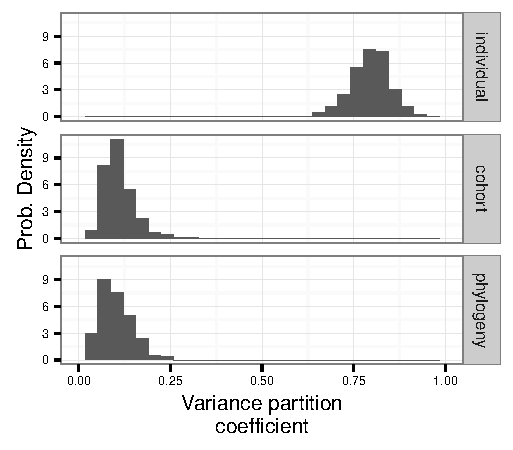
\includegraphics[height=0.3\textheight,width=\textwidth,keepaspectratio=true]{chapter_death_taxa/figure/variance_est}
  \caption[Partitioned variance for mammal survival]{Estimates of the variance partitioning coefficients for the three different sources of variance: species, cohort, and phylogeny. Higher values correspond to greater contribution to total observed variance. Each of the estimates is a distribution of 1000 approximating simulations due to the model's non-normally distributed errors.}
  \label{fig:vpc}
\end{figure}

Of the three sources of variance present in the model, individual species variance accounts for approximately 80\% of the observed, unmodeled variance (Fig.~\ref{fig:vpc}). Note that the individual variance was approximated using an simulation approach \cite{Goldstein2002} because the Weibull distribution does not have a variance term. Both cohort and phylogenetic effects account for the other 20\% of the observed variance. This result means that extinction risk has both temporal and phylogenetic aspects, as both contribute greater than 0\% of the observed variability in the data \cite{Housworth2004}. 


% decrease in extinction risk with time is known previous result
% plot S(t) for each cohort with posterior predictive checks as panels?
%   this is probably very useful way of depicting variance in cohort survival functions
% two part figure 
%   Exponential and Weibull fit to S(t)
%   facet grid with each cohort S(t)
%     show Exponential and Weibull fits per cohort, two overlaping colors

\begin{figure}[ht]
  \centering
  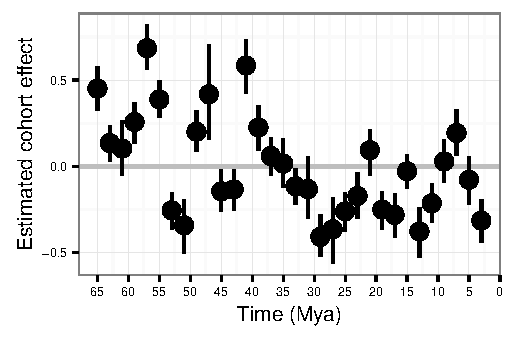
\includegraphics[height=0.4\textheight,width=\textwidth,keepaspectratio=true]{chapter_death_taxa/figure/cohort_est}
  \caption[Effect of cohort on mammal survival]{Summaries of posterior estimates of individual cohort effect depicted as medians and 80\% credible intervals. High values correspond to shorter species durations while lower values correspond to greater species durations compared to the mean duration. Lines are placed at the middle of the 2 My origination cohorts.}
  \label{fig:eff_cohort}
\end{figure}

The estimates for the individual cohort effects show a weak pattern of greater extinction risk in older Cenozoic cohorts compared to younger cohorts (Fig.~\ref{fig:eff_cohort}). This potential slowdown in extinction risk is consistent with previous analyses of marine invertebrates \cite{Raup1982a,Foote2003} and mammals \cite{Alroy2010c,Alroy2000g}. There are two prevailing hypotheses as to the cause of this slowdown: 1) extinction risk is constant within, but varies between, clades so over time clades with low extinction rates increases in proportion of total diversity thus bringing down expected extinction risk; or 2) over time taxa increase in mean fitness and thus decrease in expected extinction risk \cite{Raup1982a}. The observed decrease in extinction risk with age, along with the variance partitioning results (Fig.~\ref{fig:vpc}) are consistent with both of these hypotheses with neither being more ``important'' than the other. 

Interestingly, the shift from older cohorts with a higher extinction risk to younger cohorts with lower extinction risk is approximately at the Paleogene--Neogene boundary. Given the association with arboreality and increased extinction risk (Fig.~\ref{fig:trait_est}), the decrease in expected extinction risk over time might relate to the preferential loss of arboreal taxa over the Cenozoic. However, because the model used here does not allow for time-varying effects, I cannot identify whether this boundary is associated with a shift in the direction or magnitude of the expected effect of arboreality on extinction risk.

\section{Discussion}
My results indicate that Cenozoic North American mammal ``generalists'' are expected to have a lower extinction risk than ``specialists.'' This implies that the diversification of specialized taxa would have required either a driven trend away from generality \cite{McShea1994} or an increase in speciation rate relative to extinction rate \cite{Stanley1975}. This requires that specialist traits should somehow increase or be associated with increases in speciation rate, perhaps via niche partitioning or changes in habitat heterogeneity. For example, descendant species of omnivores many divide available prey items more finely or arboreal taxa may increase in both extinction and speciation rates via increases in habitat heterogeneity. Possible evidence to support this hypothesis would be to demonstrate differences in speciation rate associated with those traits analyzed here or other similar traits.

When these results are compared to factors contributing to increased extinction risk in extant mammals, there are some incongruencies. As expected, large range size is consistently associated with lower extinction risk in the modern world \cite{Liow2009,Purvis2000a,Fritz2009,Fritz2010b}. While my analysis found body size to have almost no time-invariant effect on extinction risk, in extant mammals this is not necessarily the case as increased body size is associated with increased extinction risk \cite{Liow2009,Purvis2000a}. However, this pattern is partially clade dependent \cite{Fritz2009}. As stated earlier, higher trophic levels have been found to be associated with greater extinction risk in extant mammals \cite{Liow2009,Purvis2000a}. In contrast, I found that omnivores and carnivores have a lower expected extinction risk than either insectivores or herbivores (Fig.~\ref{fig:trait_est}). Finally, phylogeny has been found to be a good predictor of differences in extinction risk in extant mammals as certain clades are at much higher risks than others \cite{Fritz2010b}. This effect seems much greater in the Recent than for the whole Cenozoic, implying that current extinction risk is more phylogenetically concentrated than during times of background extinction levels during the Cenozoic.

Whether these incongruities are within the standard range of time-variant effects is unknown, though my comparisons do imply that current processes are different from those studied here. However, this is not a model of what makes taxa vulnerable during mass extinctions and that may account for these incongruities, assuming mass extinctions are qualitatively different than background extinction \cite{Jablonski1986}. These results would also be inapplicable if the current biodiversity crisis is qualitatively different from either background or mass extinction as preserved in the fossil record.

By modeling how different ecologies and historical factors effect a species' expected extinction risk, it is possible to better understand what processes may have driven the resulting pattern of selection (i.e. diversity) while also providing a baseline for evaluating the current biodiversity crisis. This analysis finds support for the ``survival of the unspecialized'' hypothesis \cite{Simpson1944,Liow2004a} as a time-invariant generalization about extinction risk. I also find that there are substantial effects of both cohort and phylogeny on extinction risk, which supports the idea that the decrease in extinction risk \cite{Raup1982a} over time has both temporal and phylogenetic components. Additionally, I found evidence of increasing extinction risk with species age, the cause of which is unknown. These results show that, like prior mass extinction events in the fossil record, the current biodiversity crisis is qualitatively different from the previous period of background extinction in the fossil record \cite{Jablonski1986}.


%\begin{materials}
\section{Materials and Methods}
\subsection{Species occurrence and covariate information}
Fossil occurrence information was downloaded from the Paleobiology Database (PBDB; http://paleodb.org/). Occurrence, taxonomic, stratigraphic, and biological information was downloaded for all North American mammals. This data set was filtered so that only occurrences identified to the species-level, excluding all ``sp.''-s. All aquatic and volant taxa were also excluded. Additionally, all occurrences without latitude and longitude information were excluded from the sample.


\begin{table}[ht]
  \centering
  \caption[Cypher for ecotype assignments]{Species trait assignments in this study are a coarser version of the information available in the PBDB. Information was coarsened to improve per category sample size and uniformity and followed this table.}
  \begin{tabular}[ht]{ l | l | l }
    \hline
    \multicolumn{2}{ c |}{This study} & PBDB categories \\
    \hline \hline
    \multirow{4}{*}{Diet} & Carnivore & Carnivore \\
    & Herbivore & Browser, folivore, granivore, grazer, herbivore. \\
    & Insectivore & Insectivore. \\
    & Omnivore & Frugivore, omnivore. \\ 
    \hline
    \multirow{3}{*}{Locomotor} & Arboreal & Arboreal.\\
    & Ground dwelling & Fossorial, ground dwelling, semifossorial, saltatorial. \\
    & Scansorial & Scansorial. \\
    \hline
  \end{tabular}
  \label{tab:trait_cats}
\end{table}

Species dietary and locomotor category assignments were done using the assignments in the PBDB, which were reassigned into coarser categories (Table \ref{tab:trait_cats}). This was done to improve interpretability, increase sample size per category, and make results comparable to previous studies \cite{Jernvall2004,Price2012}.


All individual fossil occurrences were assigned to 2 My bins ranging through the entire Cenozoic. Taxon duration was measured as the number of 2 My bins from the first occurrence to the last occurrence, inclusive. This bin size was chosen because it approximately reflects the resolution of the North American Cenozoic mammal fossil record \cite{Alroy2009,Alroy2000g,Marcot2014}. Species originating in the youngest cohort, 0-2 My, were excluded from analysis because every species duration would be both left and right censored, which is illogical.

\begin{table}[ht]
  \centering
  \caption[Equations used to estimate mammal mass]{Regression equations used in this study for estimating body size. Equations are presented with reference to taxonomic grouping, part name, and reference.}
  \begin{tabular}{l | l | l | l}
    Group & Equation & log(Measurement) & Source \\
    \hline
    General & \(\log(m) = 1.827x + 1.81\) & lower m1 area &  \cite{Legendre1986} \\
    General & \(\log(m) = 2.9677x - 5.6712\) & mandible length & \cite{Foster2009a} \\
    General & \(\log(m) = 3.68x - 3.83\) & skull length & \cite{Luo2001} \\
    Carnivores & \(\log(m) = 2.97x + 1.681\) & lower m1 length & \cite{VanValkenburgh1990} \\
    Insectivores & \(\log(m) = 1.628x + 1.726\) & lower m1 area & \cite{Bloch1998} \\
    Insectivores & \(\log(m) = 1.714x + 0.886\) & upper M1 area & \cite{Bloch1998} \\
    Lagomorph & \(\log(m) = 2.671x - 2.671\) & lower toothrow area & \cite{Tomiya2013} \\
    Lagomorph & \(\log(m) = 4.468x - 3.002\) & lower m1 length & \cite{Tomiya2013} \\
    Marsupials & \(\log(m) = 3.284x + 1.83\) & upper M1 length & \cite{Gordon2003} \\
    Marsupials & \(\log(m) = 1.733x + 1.571\) & upper M1 area & \cite{Gordon2003} \\
    Rodentia & \(\log(m) = 1.767x + 2.172\) & lower m1 area & \cite{Legendre1986} \\
    Ungulates & \(\log(m) = 1.516x + 3.757\) & lower m1 area & \cite{Mendoza2006} \\
    Ungulates & \(\log(m) = 3.076x + 2.366\) & lower m2 length & \cite{Mendoza2006} \\
    Ungulates & \(\log(m) = 1.518x + 2.792\) & lower m2 area & \cite{Mendoza2006} \\
    Ungulates & \(\log(m) = 3.113x - 1.374\) & lower toothrow length & \cite{Mendoza2006} \\
    \hline
  \end{tabular}
  \label{tab:mass_est}
\end{table}

Species body size estimates in grams were sourced from a large selection of primary literature and database compilations. Databases used include the PBDB, PanTHERIA \cite{Jones2009c}, and the Neogene Old World Mammal database (NOW; http://www.helsinki.fi/science/now/). Major sources of additional compiled body size estimates include \cite{Tomiya2013,Brook2004a,Freudenthal2013,McKenna2011,Raia2012f,Smith2004c}. These were then supplemented with an additional literature search to try and fill in the remaining gaps. In many cases, species body mass was estimated using various published regression equations based on tooth or skull measurements (Table \ref{tab:mass_est}). If multiple specimens were measured, I used the mean of specimen measures as the species mean. See Dataset S1 for a complete list of mass estimates and sources. \uppercase{fix me}



\subsubsection{Biogeographic network}
Species geographic extent was measured as the mean of the relative number of bioprovinces occupied by a species for each 2 My bin the species was present. Bioprovinces were identified using a network-theoretic approach that has previously been applied to paleontological data \cite{Sidor2013,Vilhena2013}. This approach relies on defining a biogeographic bipartite network of taxa and localities. In this study, taxa were defined as species and localities were grid cells from a regular lattice on a global equal-area cylinder map projection. The regular lattice was defined as a 70 x 34 global grid where each cell corresponds to approximately 250000 km\(^{2}\). An advantage of this approach is that this approach reduces to occupancy when all localities are independent and to a single bioprovince when all localities are identical.

A biogeographic network was constructed for each of the 2 My bins used in this study. Emergent bioprovinces were then identified using the map equation \cite{Rosvall2008,Rosvall2009a} as has been done before \cite{Sidor2013,Vilhena2013b,Vilhena2013}. These bioprovinces correspond to taxa and localities that are more interconnected with each other than with other nodes.

The map projection and regular lattice were made using shape files from \\http://www.naturalearthdata.com/ and the \texttt{raster} package for R \cite{raster}. Bioprovince identification was done using the map equation as implemented in the \texttt{igraph} package for R \cite{csardi2006igraph}.


\subsubsection{Supertree}
As there is no single, combined formal phylogenetic hypothesis of all Cenozoic fossils mammals from North America, it was necessary to construct a semi-formal supertree. This was done by combining taxonomic information for all the observed species and a few published phylogenies using matrix representation parsimony \cite{Bininda-Emonds2007}. For further explanation of the methodology used to construct this supertree, please see the Supplementary information in Section \ref{sec:death_taxa_supp}.


\subsection{Survival model}
Presented here is the model development process used to formulate the two survival models used in this study. First, define \(y\) as a vector of length \(n\) where the \(i\)th element is the duration of species \(i\), where \(i = 1,\cdots,n\).

The simplest survival model where durations are assumed to follow an exponential distribution with a single ``rate'' or inverse-scale parameter \(\lambda\) \cite{Klein2003}. This is written
\begin{align}
  p(y | \lambda) &= \lambda \exp(-\lambda y) \nonumber \\
  y &\sim \mathrm{Exp}(\lambda).
  \label{eq:exp}
\end{align}
The exponential distribution corresponds to situations where extinction risk is independent of age. To understand this, we need to define two functions: the survival function \(S(t)\) and the hazard function \(h(t)\). \(S(t)\) is the probability that a species having existed for \(t\) 2 My bins will not have gone extinct while \(h(t)\) corresponds to the instantaneous extinction rate for some taxon age \(t\) \cite{Klein2003}. For an exponential model, \(S(t)\) is 
\begin{equation}
  S(t) = \exp(-\lambda t)
  \label{eq:exp_surv}
\end{equation}
and \(h(t)\) is defined
\begin{equation}
  h(t) = \lambda
  \label{eq:exp_haz}
\end{equation}
The choice of the exponential distribution corresponds directly to the Law of Constant Extinction \cite{VanValen1973} as the right side of Eq.~\ref{eq:exp_haz} does not depend on species age \(t\). 

The current sampling statement (Eq.~\ref{eq:exp}) assumes that all species share the same rate parameter with no variation. To allow for variation in \(\lambda\) associated with relevant covariate information like species body size, \(\lambda\) is reparameterized as \(\lambda_{i} = \exp(\sum \beta^{T}\mathbf{X}_{i})\) with \(i\) indexing a given observation and its covariates, \(\beta\) is a vector of regression coefficients, and \(\mathbf{X}\) is a matrix of covariates. This is a standard regression approach, where one column of \(\mathbf{X}\) is all 1-s and its corresponding \(\beta\) coefficient is the intercept. 

\(\mathbf{X}\) is an \(n \times K\) matrix of species-level covariates. Three of the covariates of interest are the logit of mean relative occupancy, and the logarithm of body size (g). The discrete covariate index variables of dietary and locomotor category were transformed into \(n \times (k - 1)\) matrices where each column is an indicator variable (0/1) for that species's category, \(k\) being the number of categories of the index variable (3 and 4, respectively). Only \(k - 1\) indicator variables are necessary as the intercept takes on the remaining value. For example, the difference in effect of arboreality versus scansoriality on extinction risk, given that arboreality is the reference category, is the coefficient for the scansorial indicator variable as that is the difference between between the effect of arboreality (the intercept \(\beta_{0}\)) and scansoriality (the intercept + scansorial effect \(\beta_{s}\)); Fig. \ref{fig:trait_est}). Finally, a vector of 1-s was included in the matrix \(\mathbf{X}\) whose corresponding \(\beta\) coefficient is the intercept, making \(K\) equal eight.

\(\beta\) is the vector of regression coefficients. The intercept term was given a weak normal prior, \(\beta_{0} \sim \mathcal{N}(0, 10)\) while all of these other coefficients were slightly more informative priors, e.g. \(\beta_{mass} \sim \mathcal{N}(0, 5)\). These priors were chosen because it is expected that the effect size of each variable on duration will be small, as is generally the case with binary covariates \cite{Gelman2007}.

Regression coefficients are not directly comparable without first standardizing the input variables to have equal standard deviations. This is accomplished by subtracting the mean of the covariate from all values and then dividing by the standard deviation, resulting in a variable with mean of zero and a standard deviation of one. This linear transform greatly improves the interpretability of the coefficients as expected change in mean duration given a difference of one standard deviation in the covariate \cite{Schielzeth2010}. Additionally, this makes the intercept directly interpretable as the estimate of mean (transformed) \(\sigma\) (Eq.~\ref{eq:reg}). However, because the expected standard deviation for a random binary variable is 0.5, in order to make comparisons between the binary and continuous variables, the continuous inputs were divided by twice their standard deviation \cite{Gelman2008}. 

Origination cohort is defined as the group of species which all originated during the same 2 My temporal bin. Because the most recent temporal bin, 0-2 My, was excluded, there are 32 total cohorts. The effect of origination cohort \(j\) was modeled with each group being a sample from a common cohort effect, \(\eta\), which was considered normally distributed with mean 0, and standard deviation \(\sigma_{c}\). The value of \(\sigma_{c}\) was then estimated from the data itself, corresponding to the amount of pooling in the individual estimates of \(\eta_{j}\). This approach is a conceptual and statistical unification between dynamic and cohort survival analysis in paleontology \cite{Foote1988,Raup1978,Raup1975,VanValen1979,Baumiller1993}, with \(\sigma_{c}\) acting as a measure of compromise between these two end members. The choice of the half-Cauchy prior for \(\sigma_{c}\) follows \cite{Gelman2006a}.
\begin{align*}
  \eta_{j} &\sim \mathcal{N}(0, \sigma_{c}) \\
  \sigma_{c} &\sim \mathrm{C}^{+}(0, 2.5)
\end{align*}

The impact of shared evolutionary history, or phylogeny, was modeling as an individual effect where each observation, \(i\), is modeled as a multivariate normal, \(h\), where the covariance matrix \(\Sigma\) is known up to a constant, \(\sigma_{p}^{2}\) \cite{Lynch1991,Housworth2004}. This is written
\begin{align*}
  h &\sim \mathrm{MVN}(0, \mathbf{\Sigma}) \\
  \mathbf{\Sigma} &= \sigma_{p}^{2} \mathbf{V}_{phy} \\
  \sigma_{p} &\sim \mathrm{C}^{+}(0, 2.5).
\end{align*}

\(\mathbf{V}_{phy}\) is the phylogenetic covariance matrix defined as an \(n \times n\) matrix where the diagonal elements are the distance from root to tip, in branch length, for each observation and the off-diagonal elements are the amount of shared history, measured in branch length, between observations \(i\) and \(j\). \(\sigma_{p}\) was given a weakly informative half-Cauchy hyperprior. Note that because the phylogeny used here is primarily based on taxonomy, estimates of \(\sigma_{p}\) represent minimum estimates \cite{Lynch1991,Housworth2004}. Improved phylogenetic estimates of all fossil Cenozoic mammals would greatly improve this estimate.

To relax the assumption of age-independent extinction of the Law of Constant Extinction, the Weibull distribution is substituted for the exponential \cite{Klein2003}. The Weibull distribution has a shape parameter \(\alpha\) and scale parameter \(\sigma\). Conceptually, \(\sigma\) is the inverse of \(\lambda\). \(\alpha\) modifies the impact of taxon age on extinction risk. When \(\alpha > 1\) then \(h(t)\) is a monotonically increasing function, but when \(\alpha < 1\) then \(h(t)\) is a monotonically decreasing function. When \(\alpha = 1\) then the Weibull distribution is equivalent to the exponential.

The Weibull distribution and sampling statement were defined
\begin{align}
  p(y | \alpha, \sigma) &= \frac{\alpha}{\sigma} \left(\frac{y}{\sigma}\right)^{\alpha - 1} \exp\left(-\left(\frac{y}{\sigma}\right)^{\alpha}\right) \nonumber \\
  y &\sim \mathrm{Weibull}(\alpha, \sigma).
  \label{eq:weibull}
\end{align}
The corresponding \(S(t)\) and \(h(t)\) functions are defined
\begin{align}
  S(t) &= \exp\left(-\left(\frac{t}{\sigma}\right)^{\alpha}\right) \label{eq:wei_surv} \\
  h(t) &= \frac{\alpha}{\sigma}\left(\frac{t}{\sigma}\right)^{\alpha - 1} \label{eq:wei_haz}.
\end{align}

To allow for \(\sigma\) to vary with a given observation's covariate information it is reparameterized in a similar fashion to \(\lambda\) with a few key differences. Because \(\sigma = 1/\lambda\) in order to preserve the interpretation of \(\beta\), while taking \(\alpha\) into account, \(\sigma\) is reparameterized as
\begin{equation}
  \sigma_{i} = \exp\left(\frac{-\beta}{\alpha}\right).
  \label{eq:reg}
\end{equation}

Given the above, the survival model was then fit in a Bayesian context using both exponential and Weibull distributions. The Weibull's \(\alpha\) parameter was assumed constant across species, which is standard practice in survival analysis \cite{Klein2003}. \(\alpha\) was given a weakly informative half-Cauchy (C\(^{+}\)) prior. \(\sigma\) was reparameterized as an exponentiated regression model (Eq.~\ref{eq:reg}). This was further expanded (Eq.~\ref{eq:wei_reg_ext}) to allow for two hierarchical factors as discussed above. This is written
\begin{equation}
  \sigma_{i} = \exp\left(\frac{-(h_{i} + \eta_{j[i]} + \sum \beta^{T} \mathbf{X}_{i})}{\alpha}\right)
  \label{eq:wei_reg_ext}
\end{equation}
where equivalent statement for the exponential distribution is defined
\begin{equation}
  \lambda_{i} = \exp\left(h_{i} + \eta_{j[i]} + \sum \beta^{T} \mathbf{X}_{i})\right).
  \label{eq:exp_reg_ext}
\end{equation}

An important part of survival analysis is the inclusion of censored observations where the failure time has not been observed \cite{Ibrahim2001,Klein2003}. The most common censored observation is right censored, where the point of extinction had not yet been observed in the period of study, such as taxa that are still present in the most recent time bin (0-2 My). Left censored observations, on the other hand, correspond to observations that went extinct any time between 0 and some known point. To account for this uncertainty, the probability of a left censored observation is found by integrating over all possible durations between 0 and 1 time bin. For an explanation of how censored observations are included in the sampling statement, please see the Supplementary information in Section \ref{sec:death_taxa_supp}.


\subsection{Estimation}
Parameter posteriors were approximated using a Markov-chain Monte Carlo (MCMC) routine implemented in the Stan programming language \cite{2014stan}. Stan implements a version of Hamiltonian Monte Carlo called the No-U-Turn sampler \cite{Hoffman-Gelman:2011}. Posterior approximation was done using four parallel MCMC chains run for 30000 steps, thinned to every thirtieth sample, split evenly between warm-up and sampling. Convergence was evaluated using the scale reduction factor, \(\hat{R}\). Values of \(\hat{R}\) close to 1, or less than or equal to 1.1, indicate approximate convergence. Convergence means that the chains are approximately stationary and the samples are well mixed \cite{Gelman2013d}.


\subsection{Posterior evaluation}
The most basic assessment of model fit is that simulated data generated given the model should be similar to the observed. This is the idea behind posterior predictive checks. Using the covariates from each of the observed durations, and randomly drawn parameter estimates from their marginal posteriors, a simulated data set \(y^{rep}\) was generated. This process was repeated 1000 times and the distribution of \(y^{rep}\) was compared with the observed \cite{Gelman2013d}. For results from the posterior predictive tests used in this study, please see the Supplementary information in Section \ref{sec:death_taxa_supp}.

The exponential and Weibull models were compared for out-of-sample predictive accuracy using the widely-applicable information criterion (WAIC) \cite{Watanabe2010a}. Because the Weibull model reduces to the exponential model when \(\alpha = 0\), our interest is not in choosing between these models. Instead comparison of WAIC values is useful for better understanding the effect of model complexity on out-of-sample predictive accuracy. An explanation of how WAIC is calculated is presented in the Supplementary information (Section \ref{sec:death_taxa_supp}) following the recommended ``WAIC 2'' formulation \cite{Gelman2013d}.

There are three different variance components in this model: sample component, cohort \(\sigma_{c}^{2}\), and phylogenetic \(\sigma_{p}^{2}\). Partitioning the variance between these sources allows the relative amount of unexplained variance of the sample to be compared. The sample component is similar to the residual variance from a normal linear regression. However, the Weibull based model used here (Eq.~\ref{eq:weibull}) does not include an estimate of the variance similar to the squared scale term of the a Normal distribution. Instead, the sample component was approximated via a simulation approach modified from \cite{Goldstein2002}. For explanation of this method, please see Supplementary information (Section \ref{sec:death_taxa_supp}).

I used variance partitioning coefficients (VPC) to estimate the relative importance of the different variance components \cite{Gelman2007}. Phylogenetic heritability, \(h_{p}^{2}\) \cite{Lynch1991,Housworth2004}, is identical to the VPC of the phylogenetic effect. Phylogenetic heritability is a measure of how shared evolutionary history impacts differences in individual species trait values (e.g. duration). This is a broad sense ``heritability'' as it combines both genetic inheritance and other, non-genetic shared history factors. Importantly, because phylogenetic effect was estimated using a principally taxonomy based tree the estimates derived here can be considered minimum estimates of the phylogenetic effect.


% supplement
\section{Supplemental information for ``Death and taxa''} \label{sec:death_taxa_supp}

\begin{figure}[ht]
  \centering
  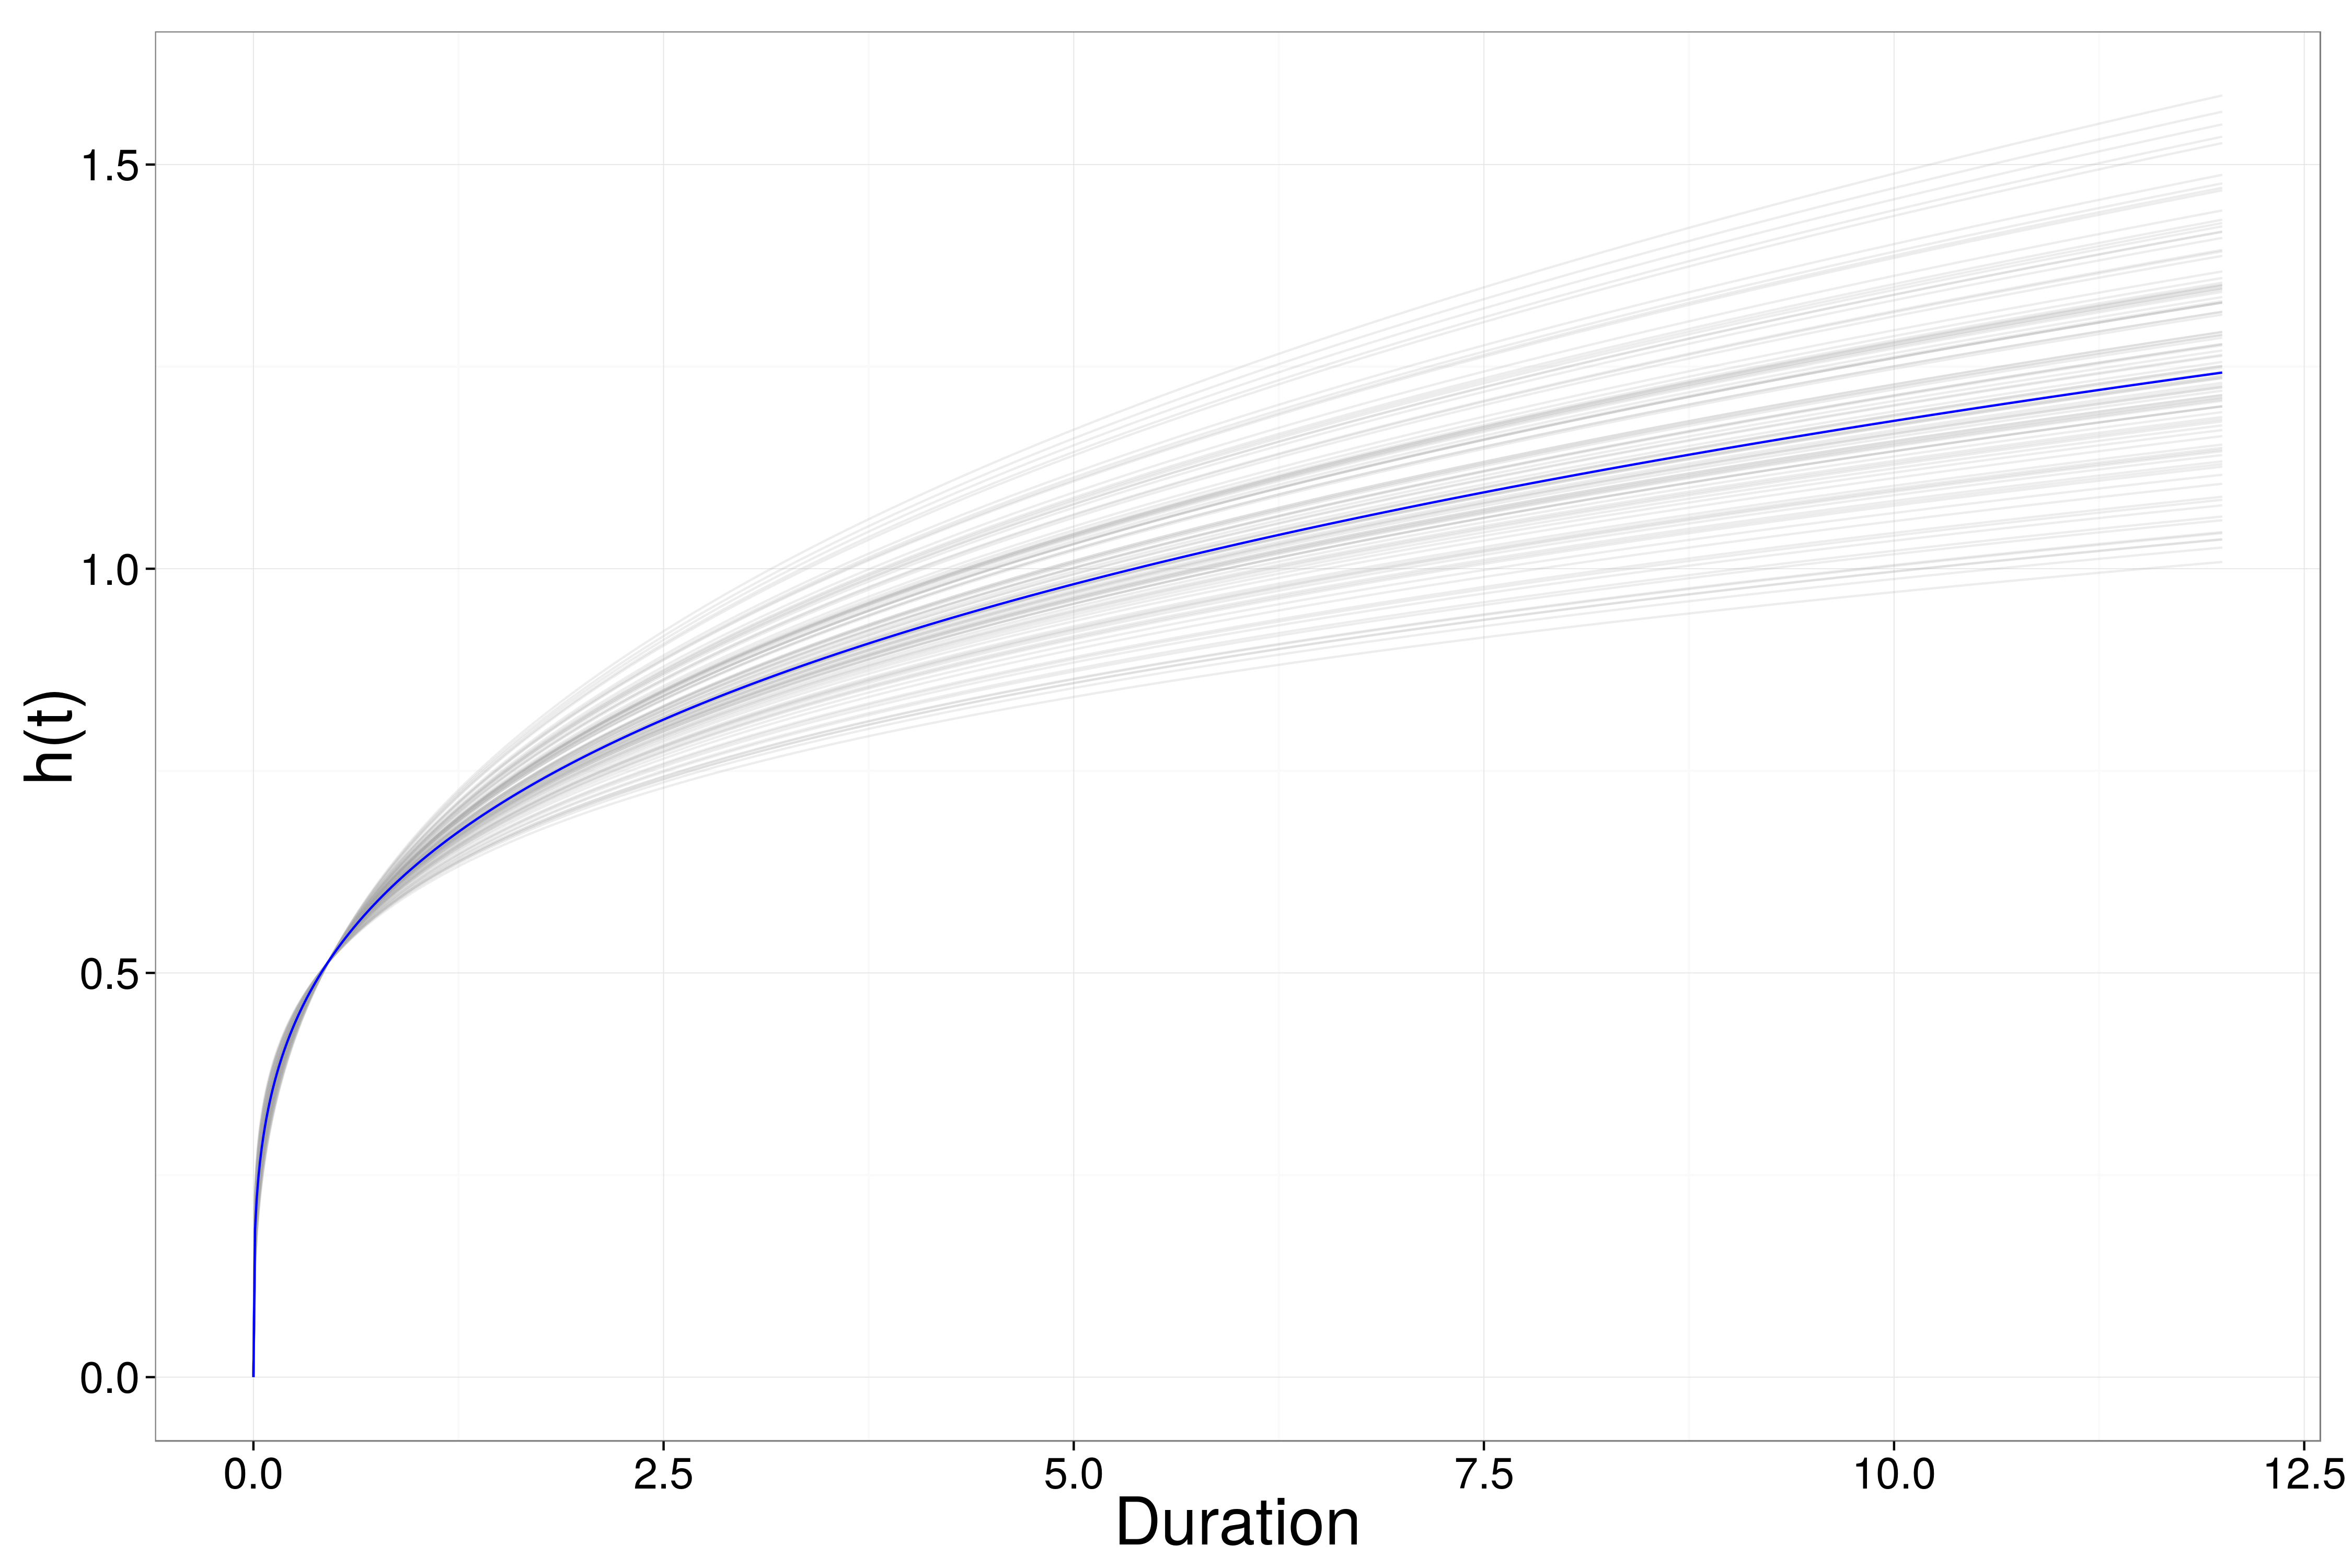
\includegraphics[height = 0.3\textheight, width = \textwidth, keepaspectratio = true]{chapter_death_taxa/figure/haz_est}
  \caption[Estimate of hazard function for mammal survival]{1000 estimates of the hazard function (\(h(t\)) for the observed species mean (grey), along with the median estimated hazard function (blue). \(h(t)\) is an estimate of the rate at which a species of age \(t\) is expected to go extinct. Hazard functions were estimated from random draws from the estimated posterior distributions and evaluated with all covariate information set to 0, which corresponds to the expected duration of the mean species.}
  \label{fig:haz}
\end{figure}


\subsection{Supertree inference}
As there is no single, combined formal phylogenetic hypothesis of all Cenozoic fossils mammals from North America, it was necessary to construct a semi-formal supertree. This was done by combining taxonomic information for all the observed species and a few published phylogenies. 

The initial taxonomic classification of the observed species was based on the associated taxonomic information from the PBDB. This information was then updated using the Encyclopedia of Life (http://eol.org/) which collects and collates taxonomic information in a single database. This was done programatically using the \texttt{taxize} package for R \cite{2013taxize}. Finally, this taxonomic information was further updated using a published taxonomy of fossil mammals \cite{Janis1998,Janis2008}. 

This taxonomy serves as an initial phylogenetic hypothesis which was then combined with a selection of species-level phylogenies \cite{Bininda-Emonds2007,Raia2012f} in order to better constrain a minimum estimate of the actual phylogenetic relationships of the species. The supertree was inferred via matrix representation parsimony implemented in the \texttt{phytools} package for R \cite{revell2012phytools}. Of the two most parsimonious trees found, I used only one for analysis.

Polytomies were resolved in order of species first appearance in order to minize stratigraphic gaps. The resulting tree was then time scaled using the \texttt{paleotree} package via the ``minimum branch length'' approach with a minimum length of 0.1 My \cite{Bapst2012a}. The minimum length is necessary to avoid zero-length branches which cause the phylogenetic covariance matrix not to be positive definite, which is important for computation (see below). While other time scaling approaches are possible \cite{Hedman2010,Bapst2013a} this method was chosen for its simplicity and not requiring additional information about diversification rates which are the interest of this study.

\subsection{Modeling censored observations}
Censored data are modeled using the survival function of the distribution, \(S(t)\), defined earlier for the Weibull distribution (Eq. 5, 6) with \(\sigma\) defined as above (Eq. 8, 9). \(S(t)\) is the probability that an observation will survive longer than a given time \(t\). 

The likelihood of uncensored observations is evaluated as normal using equation 4 while right censored observations are evaluated at \(S(t)\) and left censored observations are evaluated at \(1 - S(t)\). Note, \(1 - S(t)\) is equivalent to the cumulative distribution function and \(S(t)\) is equivalent to the complementary cumulative distribution function \cite{Gelman2013d}.

The final sampling statement/likelihood for both uncensored and both right and left censored observations is then written
\begin{equation*}
  L \propto \prod_{i \in C} \mathrm{Weibull}(y_{i} | \alpha, \sigma) \prod_{j \in R} S(y_j | \alpha, \sigma) \prod_{k \in L} \left(1 - S(y_{k} | \alpha, \sigma)\right),
\end{equation*}
where \(C\) is the set of uncensored observations, \(R\) is the set of right censored observations, and \(L\) is the set of left censored observations.

\subsection{Deviance residuals}
% need a few definitions from the main text
In standard linear regression, residuals are defined as \(r_{i} = y_{i} - y_{i}^{est}\). For the model used here, this definition is inadequate. The equivalent values for survival analysis are deviance residuals. To define how deviance residuals are calculated, we first define the cumulative hazard function \cite{Klein2003}. Given \(S(t)\), we define the cumulative hazard function as 
\begin{equation*}
  \Lambda(t) = -log\left(S\left(t\right)\right).
\end{equation*}

Next, we define martingale residuals \(m\) as
\begin{equation*}
  m_{i} = I_{i} - \Lambda(t_i).
\end{equation*}
\(I\) is the inclusion vector of length \(n\), where \(I_{i} = 1\) means the observation is completely observed and \(I_{i} = 0\) means the observation is censored. Martingale residuals have a mean of 0, range between 1 and \(-\infty\), and can be viewed as the difference between the observed number of deaths between 0 and \(t_{i}\) and the expected number of deaths based on the model. However, martingale residuals are asymmetrically distributed, and can not be interpreted in the same manner as standard residuals. 

The solution to this is to use the deviance residuals, \(D\). This is defined as a function of martingale residuals and takes the form
\begin{equation*}
  D_{i} = \text{sign}(m_{i}) \sqrt{-2[m_{i} + I_{i}log(I_{i} - m_{i})]}.
\end{equation*}
Deviance residuals have a mean of 0 and a standard deviation of 1 by definition.

\subsection{Variance partitioning}
I calculated VPC using a resampling approach based on \cite{Goldstein2002}. The procedure is as follows:
\begin{enumerate}
  \item Simulate \(w\) (50,000) values of \(\eta\); \(\eta \sim \mathcal{N}(0, \sigma_{c})\).
  \item For a given value of \(\beta^{T} \mathbf{X}\), calculate \(\sigma^{c*}\) (Eq. 7) for all \(w\) simulations, holding \(h\) constant at 0.
  \item Calculate \(\upsilon_{c}\), the Weibull variance (Eq.~\ref{eq:wei_var}) of each element of \(\sigma^{c*}\) with \(\alpha\) drawn from the posterior estimate.
  \item Simulate \(w\) values of \(h\); \(h \sim \mathcal{N}(0, \sigma_{p})\). 
  \item For a given value of \(\beta^{T} \mathbf{X}\), calculate \(\sigma^{p*}\) (Eq. 7) for all \(w\) simulations, holding \(\eta\) constant at 0.
  \item Calculate \(\upsilon_{p}\), the Weibull variance (Eq.~\ref{eq:wei_var}) of each element of \(\sigma^{p*}\) with \(\alpha\) drawn from the posterior estimate.
  \item \(\sigma_{y*}^{2} = \frac{1}{2} \left(\left(\frac{1}{w} \sum_{i}^{w} \upsilon_{pi}\right) + \left(\frac{1}{w} \sum_{j}^{w} \upsilon_{cj}\right)\right)\).
  \item \(\sigma_{c*}^{2} = var(\upsilon_{c})\) and \(\sigma_{p*}^{2} = var(\upsilon_{p})\).
\end{enumerate}

The simulated values of \(h\) were drawn from a univariate normal distribution because each simulated value is in isolation, so there is no concern of phylogenetic autocorrelation. The chosen value for \(\beta^{T} \mathbf{X}\) was a draw from the posterior estimate of the intercept. Because input variables were standardized prior to model fitting, the intercept corresponds to the estimated effect on survival of the sample mean.

Weibull variance is calculated as
\begin{equation}
  var(x) = \sigma^{2}\left(\Gamma\left(1 + \frac{2}{\alpha}\right) - \left(\Gamma\left(1 + \frac{1}{\alpha}\right)\right)^{2}\right),
  \label{eq:wei_var} \end{equation}
where \(\Gamma\) is the gamma function. 

The variance partitioning coefficients are then calculated, for example, as \(VPC_{phylo} = \frac{\sigma_{p*}^{2}}{\sigma_{y*}^{2} + \sigma_{c*}^{2} + \sigma_{p*}^{2}}\) and similarly for the other components.



\subsection{Widely applicable information criterion}
WAIC can be considered fully Bayesian alternative to the Akaike information criterion, where WAIC acts as an approximation of leave-one-out cross-validation which acts as a measure of out-of-sample predictive accuracy \cite{Gelman2013d}. The following explanation uses the ``WAIC 2'' formulation recommended by \cite{Gelman2013d}. 

WAIC is calculated starting with the log pointwise posterior predictive density calculated as
\begin{equation}
  \mathrm{lppd} = \sum_{i = 1}^{n} \log \left(\frac{1}{S} \sum_{s = 1}^{S} p(y_{i}|\Theta^{S})\right),
  \label{eq:lppd}
\end{equation}
where \(n\) is sample size, \(S\) is the number posterior simulation draws, and \(\Theta\) represents all of the estimated parameters of the model. This is similar to calculating the likelihood of each observation given the entire posterior.

A correction for the effective number of parameters is then added to lppd to adjust for overfitting. The effective number of parameters is calculated, following derivation and recommendations of \cite{Gelman2013d}, as
\begin{equation}
  p_{\mathrm{WAIC}} = \sum_{i = 1}^{n} V_{s = 1}^{S} (\log p(y_{i}|\Theta^{S})).
  \label{eq:pwaic}
\end{equation}
where \(V\) is the sample posterior variance of the log predictive density for each data point.

Given both equations \ref{eq:lppd} and \ref{eq:pwaic}, WAIC is then calculated
\begin{equation}
  \mathrm{WAIC} = \mathrm{lppd} - p_{\mathrm{WAIC}}.
  \label{eq:waic}
\end{equation}
When comparing two or more models, lower WAIC values indicate better out-of-sample predictive accuracy. Importantly, WAIC is just one way of comparing models. When combined with posterior predictive checks it is possible to get a more complete understanding of model fit.

\subsection{Results from posterior predictive checks}
With all marginal posterior estimates having converged (\(\hat{R} < 1.1\)) it is possible to examine the quality of model fit (Table 1). If the model is an adequate descriptor of the observed data, then relatively confident inference can be made \cite{Gelman2013d}.

\begin{figure}[ht]
  \centering
  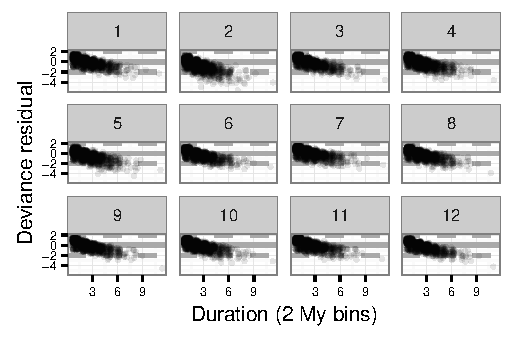
\includegraphics[height = 0.4\textheight, width = \textwidth, keepaspectratio = true]{chapter_death_taxa/figure/residual_plot}
  \caption[Deviance residuals of fitted model]{Deviance residuals from the fitted survival model compared to observed durations. Each graph depicts the residuals from single draws from the posterior distributions of all estimated parameters. Positive values indicate an underestimate of the observed duration, while negative values indicate an overestimate of the observed duration. A small amount of noise is added to each point to increase clarity. Twelve different examples are provided here to indicate consistency across multiple realizations.}
  \label{fig:ppc_res}
\end{figure}

Visual examination of the deviance residuals from twelve different sets of posterior predictive simulations indicates a systematic weakness estimating durations greater than 3 2-My bins (Fig.~\ref{fig:ppc_res}). However, the comparison of posterior predictive estimates of the 25th, 50th, and 75th quantiles to the observed indicate adequate fit. (Fig.~\ref{fig:ppc_quant}). Importantly, this indicates that the model has approximate fit for 50+\% of the data. Because, the inferred model can be inferred to be approximately adequate at capturing the observed variation.

\begin{figure}[ht]
  \centering
  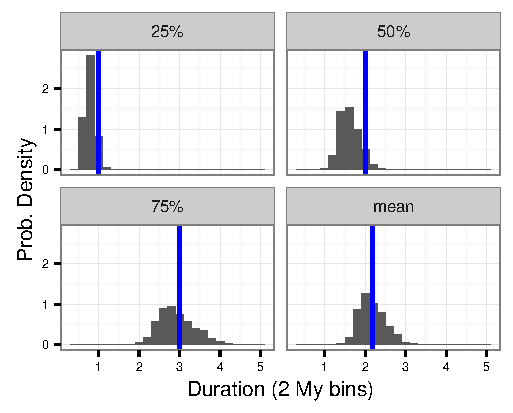
\includegraphics[height = 0.4\textheight, width = \textwidth, keepaspectratio = true]{chapter_death_taxa/figure/quant_ppc}
  \caption[Additional posterior predictive checks]{The results of additional posterior predictive checks for four summaries of the observed durations, as labeled. Blue vertical lines indicate the observed value. None of the observed values are significantly different from the posterior predictive distributions.}
  \label{fig:ppc_quant}
\end{figure}


The Wiebull model (6140.37) also had a much lower WAIC score than the Exponential model (16697.35). This large a difference indicates that the Weibull model probably has the lower out-of-sample predictive accuracy of the two.

\subsection{Data quality concerns}
A concern with using the PBDB as a primary data source, though this concerns are general to most paleontological data, is that the results are an artifact of taxonomy or the database itself \cite{Wagner2007}. However, to obtain the results obtained in this analysis there would need to be a systematic error in assignemnts of all of diet, locomotor, and taxonomic categories for a large portion of the close to 2000 sampled species. It is important to note that species included have to have body size information, much of which is found from other sources (see Dataset S1). this means that, for many taxa, that species name has to appear in occur in more than one place. this is a strong filter for misspellings and potentially invalid taxa. Additionally, given that most mammal fossils are teeth which allows for relatively accurate dietary category assignement. 

A possible concern, however, is that omnivorous taxa have feature poor morphology and thus longer durations may reflect a single anagenetic lineage as opposed to a single ``species.'' However it is possible to consider that, from a population genetic perspective, it can be argued that a single unbranching lineage is still a single biological ``unit.''

\subsection{Concerns surrounding estimates of $\alpha$}
The estimate of the Weibull shape parameter, $\alpha$, is greater than 1 meaning that extinction risk is expected to increase with taxon age (Table 1). As the value of $\alpha$ is between 1 and 1.5, extinction risk for a given species only gradually increases with age (Fig.~\ref{fig:haz}). There are three possible explanations for this result: 1) older taxa being out competed by younger taxa \cite{Wagner2014b}; or 2) this is an artifact of the minimum resolution of the fossil record \cite{Sepkoski1975}. 

An additional concern is that there may be an upward bias in estimates of $\alpha$ at this sample size, similar to that for scale parameters \cite{Gelman2013d}. The plausibility of third possibility in this example can be explored in simulation. I simulated from 10, 100, 1000, and 10000 samples from a Weibull(\(alpha = 1.3\), \(\sigma = 1\)) 100 times each. For each of these simulated datasets, I then estimated the values of \(\alpha\) and \(\sigma\) in a simple maximum likelihood context in order to just get the model estimate. The modal estimates of both parameters for the simulated datasets were then compared to the known values (Fig. \ref{fig:alpha_sims}). The results from these simulations demonstrate that the estimates of \(\alpha\) in the above analyses (Table 1) should not be particularity biased based on my sample size of approximately 2000 species. 

The model used in this analysis, however, is unable to distinguish between the remaining two hypotheses \cite{Sepkoski1975,Wagner2014b}. Further work on how to better constrain estimates $\alpha$ is necessary. A possibly is somehow incorporating these hypotheses as prior information.

\begin{figure}[ht]
  \centering
  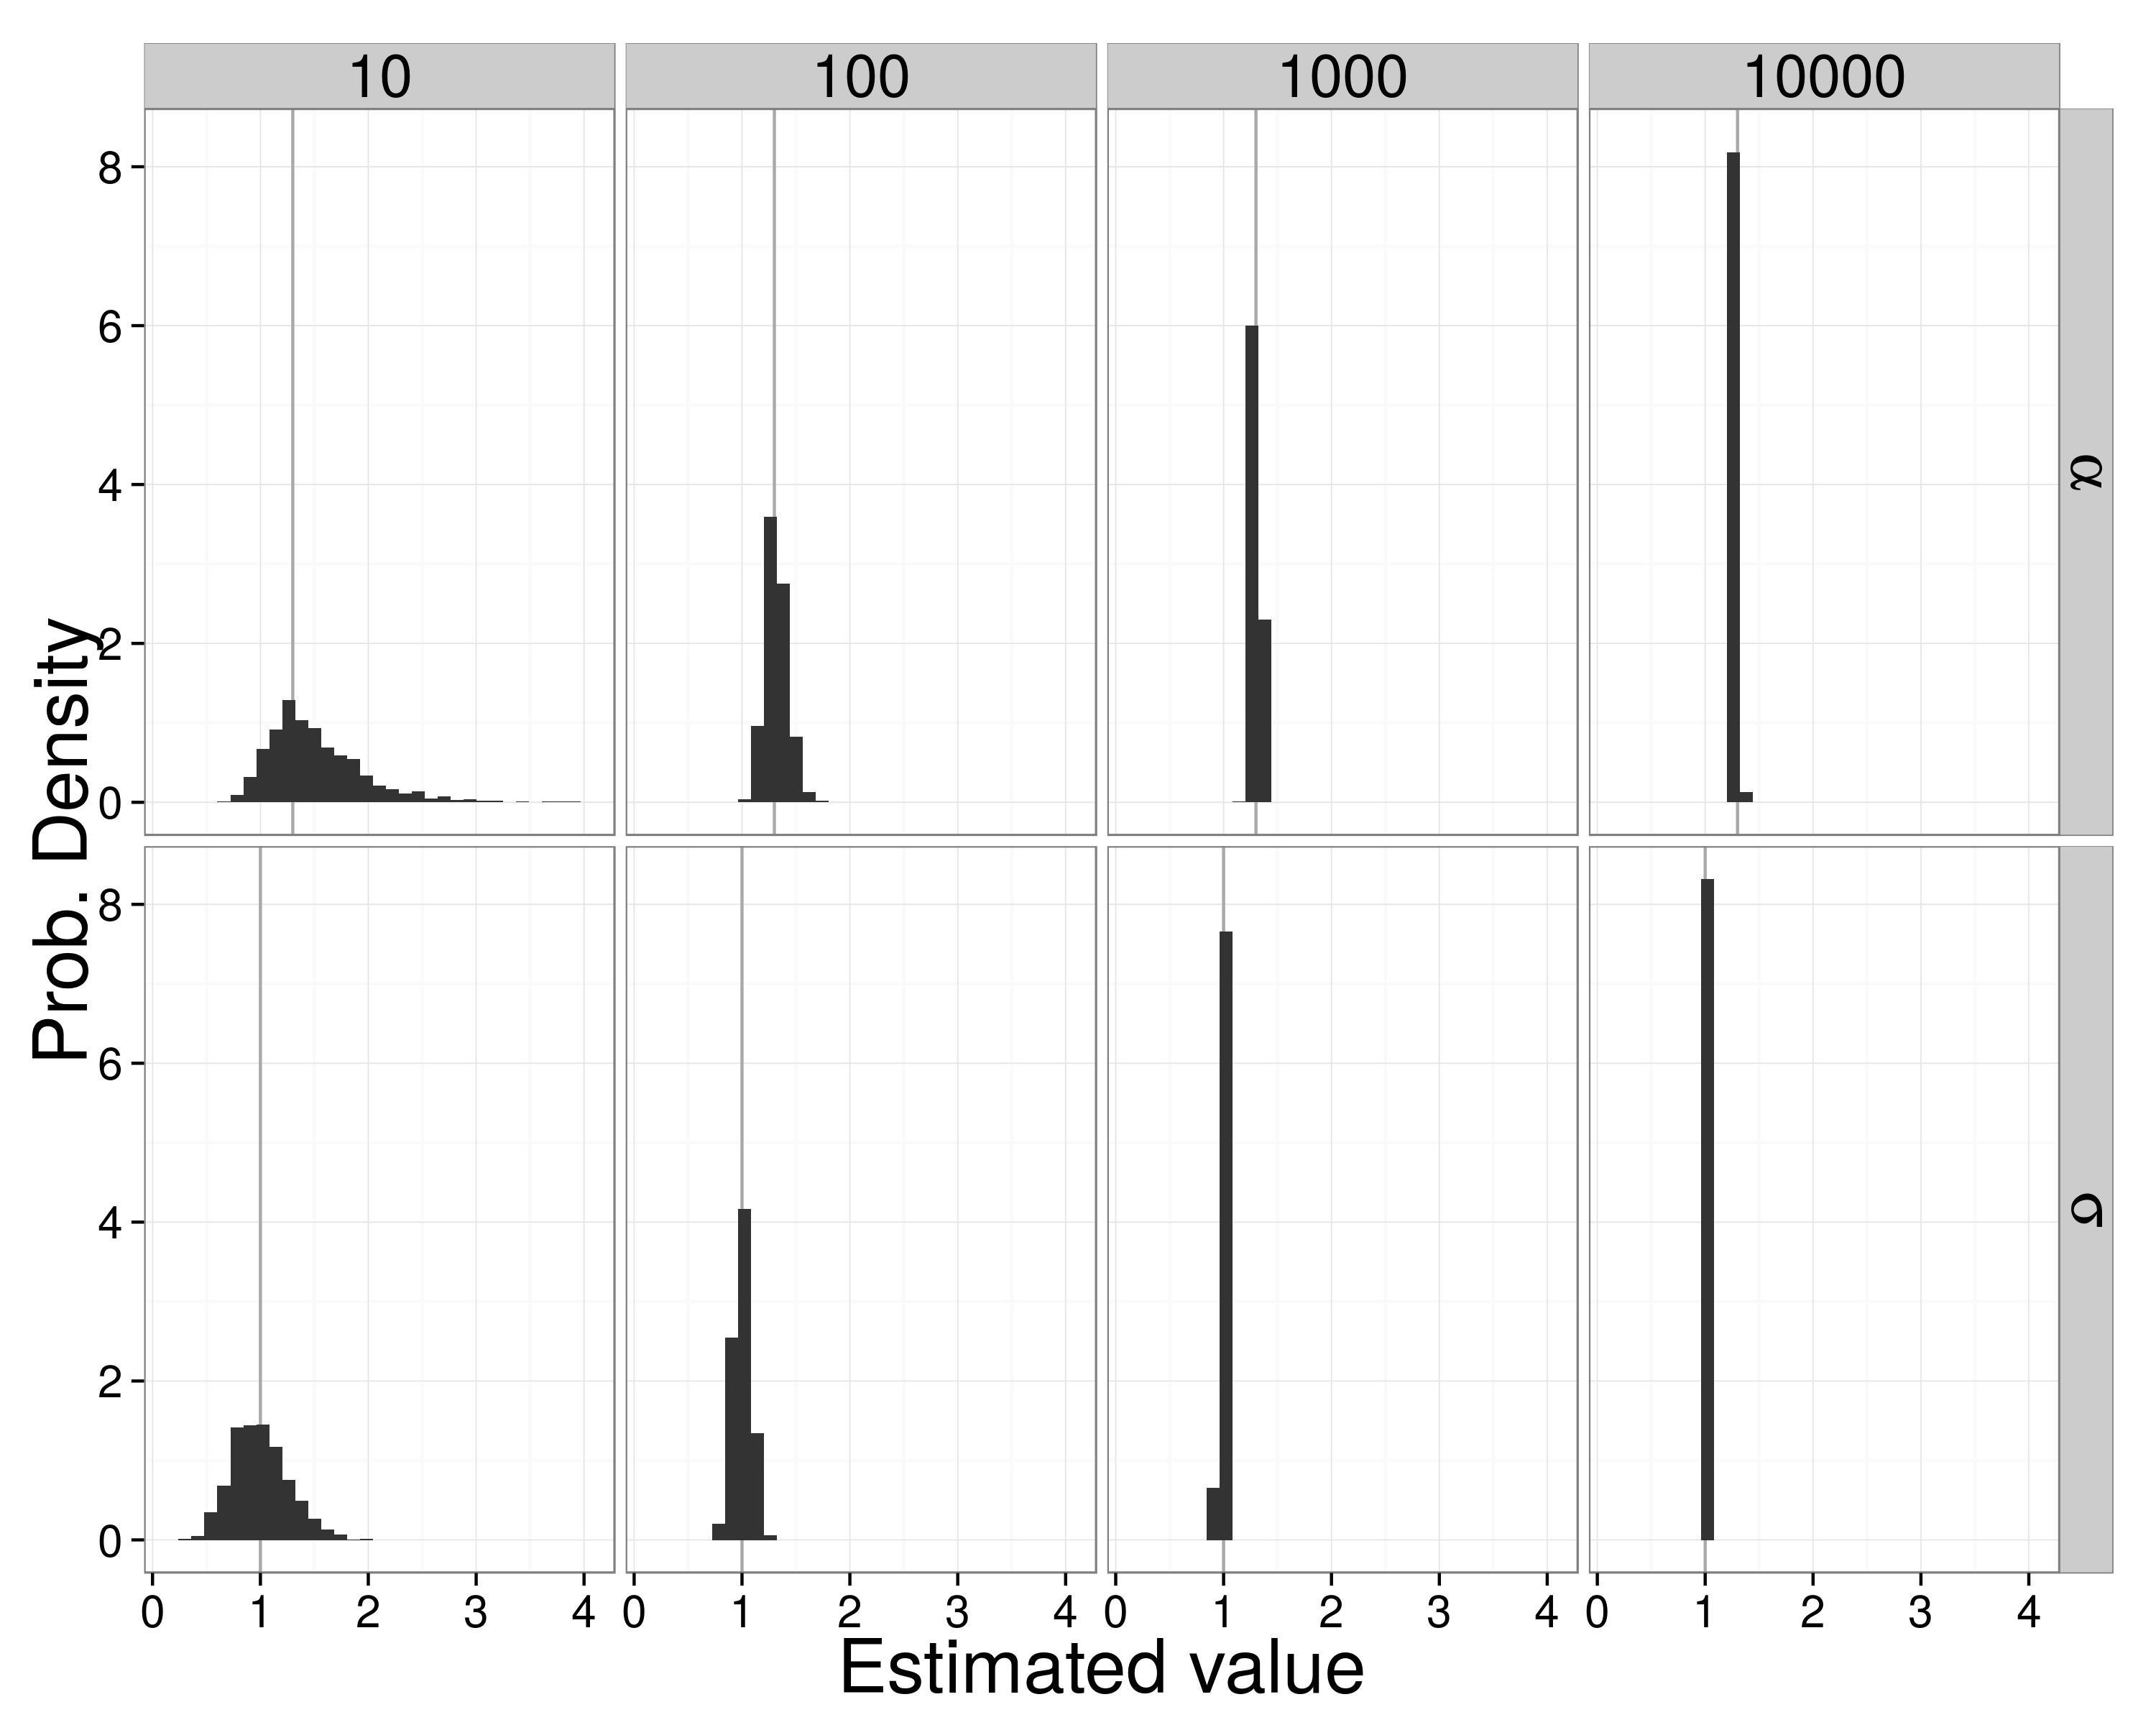
\includegraphics[height=0.4\textheight,width=\textwidth,keepaspectratio=true]{chapter_death_taxa/figure/alpha_simulation}
  \caption[Simulation of sample size and estimates of \(\alpha\)]{Comparison of maximum likelihood estimates of shape (\(\alpha\)) and scale (\(\sigma\)) parameters from 1000 simulated data sets from 4 different sample sizes. Vertical lines are the actual parameter value used to generate the data. When sample size is approximately 100 or greater, estimates are not overly biased.}
  \label{fig:alpha_sims}
\end{figure}



% chapter 2
\chapter{How macroecology affects macroevolution: the interplay between extinction intensity and trait-dependent extinction in brachiopods} \label{ch:preserve}

\begin{section_abstract}
  As extinction intensity increases, how do the effects of traits on taxonomic survival change? Does the extinction rate associated with certain traits increase while that of others decreases? Using a hierarchical Bayesian approach, I develop a model of how the effects of biological traits on extinction risk can vary with respect to extinction intensity, origination cohort (i.e. time of origination), and in relation to each other. The emergent traits traits I analyze for each brachiopod genus are geographic range, affinity for epicontinental seas versus open ocean environments, and body size. Additionally, I estimate the effects of environmental generalization versus specialization on taxonomic survival by allowing environmental preference to have a nonlinear effect on duration. My analytical framework eschews the traditional distinction between background and mass extinction, and instead considers extinction intensity as a continuum. I find that the cohort-specific effects of geographic range and environmental preference are negatively correlated with baseline extinction intensity. Additionally, I find support for greater survival of environmental generalists versus specialists in all origination cohorts. These results support the conclusion that for Paleozoic brachiopods, as extinction intensity increases overall extinction selectivity increases.
\end{section_abstract}


\section{Introduction}

Extinction is one half of the diversification process \citep{Raup1994,Stanley1979,Stanley1975}, second only to speciation or origination; it can also be the ultimate manifestation of selection as a taxon with a beneficial trait should persist for longer on average than a taxon without that beneficial trait \citep{Rabosky2010b,Jablonski2008a,Raup1994,Stanley1975}. 

While estimation of both trait-dependent speciation and extinction rates from phylogenies of extant taxa has grown dramatically \citep{Maddison2007,Fitzjohn2010,Goldberg2011a,Goldberg2005,Rabosky2013,Stadler2013b,Stadler2011a,Stadler2013a}, there are two major ways to estimate trait-dependent extinction: analysis of phylogenies, and analysis of the fossil record. These two directions, phylogenetic comparative and paleobiological, are complementary and intertwined in the field of macroevolution \citep{Rabosky2010b,Jablonski2008a,Hunt2014a}. In the case of extinction, analysis of the fossil record has the distinct advantage over phylogenies of only extant taxa because extinction is observable; this means that extinction rate is possible to estimate \citep{Rabosky2010a,Quental2009,Liow2010a}. The approach used here is thus complementary to the analysis of trait-dependent extinction based on a phylogeny.

Jabonksi \citep{Jablonski1986} observed that for bivalves at the end Cretaceous mass extinction event, the effects of some biological traits on taxonomic survival decreased. However, this pattern was not the case for the effect of geographic range on survival \citep{Jablonski1986,Payne2007}. There are multiple possible macroevolutionary mechanisms which may underlie this pattern: the effect of geographic range on survival remains constant and those of other biological traits decrease, the effect of geographic range on survival increases and those of other biological traits stay constant, or the effects of all traits decrease potentially by different degrees.

While Jablonski \citep{Jablonski1986} phrased his conclusions in terms of background versus mass extinction, these states are not distinguishable in terms of extinction rate alone; my analysis treats the time period analyzed as part of the same continuum \citep{Wang2003,Payne2007,Simpson2009}. Additionally, in order to test the proposed macroevolutionary mechanism behind this scenario \citep{Jablonski1986}; not only do the taxon trait effects need to be modeled, but the correlations between trait effects must be modeled as well. 

Here I model brachiopod taxon durations because trait based differences in extinction risk should manifest as differences in taxon durations. Brachiopods are an ideal group for this study as they are are well known for having an exceptionally complete fossil record \citep{Foote1996e,Foote2000a}. I focus on the brachiopod record from the post-Cambrian Paleozoic, from the start of the Ordovician (approximately 485 My) through the end Permian (approximately 252 My) as this represents the time of greatest global brachiopod diversity \citep{Alroy2010} meaning a large sample size for this analysis.

The analysis of taxon durations, or time from origination to extinction, falls under the purview of survival analysis, a field of applied statistics commonly used in health care and engineering \citep{Klein2003} and also has a long history in paleontology \citep{Simpson1944,Simpson1953,VanValen1973,VanValen1979,Crampton2016}. I adopt a hierarchical modeling approach \citep{Gelman2007,Gelman2013d}, which represents both a conceptual and statistical unification of the paleontological dynamic and cohort survival analytic approaches \citep{VanValen1973,VanValen1979,Raup1978,Raup1975,Foote1988,Baumiller1993,Simpson2006,Crampton2016,Ezard2012b}. 

\subsection{Factors affecting brachiopod survival}

Conceptually, taxon survival can be considered an aspect of ``taxon fitness'' \citep{Cooper1984,Palmer2012}. Traits associated with taxon survival are thus examples of species (or higher-level) selection, as differences in survival are analogous to differences in fitness. The traits analyzed here are all examples of emergent and aggregate traits \citep{Jablonski2008a,Rabosky2010b}; specifically I analyze genus-level traits. Emergent traits are those which are not measurable at a lower level (e.g. species versus individual organism) such as geographic range, or even fossil sampling rate. Aggregate traits, like body size or environmental preference, are the average of a shared trait across all members of a lower level.

Geographic range is widely considered the most important biological trait for estimating differences in extinction risk at nearly all times, with large geographic range associated with low extinction risk \citep{Jablonski1986,Jablonski1987,Jablonski2003,Payne2007,Jablonski2008a,Harnik2013,Finnegan2012a}. This stands to reason even if extinction is completely at random; a taxon with an unrestricted range is less likely to go extinct at random than a taxon with a restricted range.

Epicontinental seas are a shallow-marine environment where the ocean has spread over the continental interior or craton with a depth typically less than 100m. In contrast, open-ocean coastline environments have much greater variance in depth, do not cover the continental craton, and can persist during periods of low sea level \citep{Miller2009a}. Because of this, a simple hypothesis that taxa which favor epicontinental seas would be at great risk during periods of low sea levels, such as during glacial periods, when epicontinental seas are drained. During the Paleozoic (approximately 541--252 My), epicontinental seas were widely spread globally but declined over the Mesozoic (approximately 252--66 My) and have nearly disappeared during the Cenozoic (approximately 66--0 My) as open-ocean coastlines became the dominant shallow-marine setting \citep{Sheehan2001b,Peters2008,Miller2009a,Johnson1974}. Taxa in epicontinental environments could also have a greater extinction susceptibility than taxa in open-ocean environments due to anoxic events due to enhanced water stratification or poor water circulation \citep{Peters2007}.

Miller and Foote \citep{Miller2009a} demonstrated that during several mass extinctions taxa associated with open-ocean environments tend to have a greater extinction risk than those taxa associated with epicontinental seas. During periods of background extinction, however, they found no consistent difference between taxa favoring either environment. Miller and Foote \citep{Miller2009a} hypothesize that open-ocean taxa may have a greater extinction rate because these environments would be more strongly affected by waterborne hazards such as fallout from impacts or volcanic events which would propagate more quickly than in epicontinental environments with sluggish circulation. These two environment types represent the primary identifiable environmental dichotomy observed in ancient marine systems \citep{Miller2009a,Sheehan2001b}. Given these findings, I would hypothesize that as extinction risk increases, the extinction risk associated with open-ocean environments should generally increase. 

Because environmental preference is defined here as the continuum between occurring exclusively in open-ocean environments versus epicontinental environments, intermediate values are considered ``generalists'' in the sense that they favor neither end member. A long-standing hypothesis is that generalists or unspecialized taxa will have greater survival than specialists \citep{Simpson1944,Liow2004a,Liow2007b,Nurnberg2013a,Nurnberg2015,Baumiller1993,Smits2015b}. Because of this, the effect of environmental preference was modeled as a quadratic function where a concave down relationship between preference and expected duration indicates that generalists are favored over specialists end-members.

Body size, measured as shell length, is also considered as a trait that may potentially influence extinction risk \citep{Payne2014,Harnik2011}. Body size is a proxy for metabolic activity and other correlated life history traits \citep{Payne2014}. Harnik \textit{et al.} \citep{Harnik2014} analyzed the effect of body size selectivity in Devonian brachiopods in both a phylogenetic and non-phylogenetic context; finding that body size was not found to be associated with differences in taxonomic duration. It has also been found that, at least in the case of some bivalve subclades, body size can be as important a factor as geographic range size in determining extinction risk \citep{Harnik2011}. Given these results, I expect that if body size has any effect on brachiopod taxonomic survival it is very small.

It is well known that, given the incompleteness of the fossil record, the observed duration of a taxon is an underestimate of that taxon's true duration \citep{Solow1997,Wagner2013a,Wang2004,Liow2010b,Alroy2014a,Foote1996e}. Because of this, the concern is that a taxon's observed duration may reflect its relative chance of being sampled and not any of the effects of the covariates of interest. In this case, for sampling to be a confounding factor there must be consistent relationship between the quality of sampling of a taxon and its apparent duration (e.g. greater sampling, longer duration). If there is no relationship between sampling and duration then interpretation can be made clearly; while observed durations are obviously truncated true durations, a lack of a relationship would indicate that the amount and form of this truncation is not a major determinant of the taxon's apparent duration. By including sampling as a covariate in the model, this effect can be quantified and can be taken into account when interpreting the estimates of the effects of the other covariates.



\section{Materials and Methods}

\subsection{Fossil occurrence information}

% foote gave me a hand with the taxonomic occurrences
%   biggest limiting factor is the Payne 2014 body size dataset
The brachiopod dataset analyzed here was sourced from the Paleobiology Database \\(http://www.paleodb.org) which was then filtered based on taxonomic (Rhychonelliformea: Rhynchonellata, Chileata, Obolellida, Kutorginida, Strophomenida, Spiriferida), temporal (post-Cambrian Paleozoic), stratigraphic, and other occurrence information used in this analysis. Analyzed occurrences were restricted to those with paleolatitude and paleolongitude coordinates, assignment to either epicontinental or open-ocean environment, and belonging to a genus present in the body size dataset \citep{Payne2014}. Epicontinental versus open-ocean assignments for each fossil occurrence are partially based on those anaylzed by Miller and Foote \citep{Miller2009a}, with additional occurrences assigned similarly (Miller and Foote, personal communication). These filtering criteria are very similar to those used by Miller and Foote \citep{Foote2013} with an additional constraint of being present in the body size data set from Payne \textit{et al} \citep{Payne2014}. In total, 1130 genera included in the dataset.

% justification of using genus level versus specific
Fossil occurrences were analyzed at the genus level which is common for paleobiological, macroevolutionary and macroecological studies of marine invertebrates \citep{Alroy2010,Foote2013,Harnik2013,Kiessling2007a,Miller2009a,Nurnberg2013a,Nurnberg2015,Payne2007,Simpson2009,Vilhena2013}. While species diversity dynamics are frequently of much greater interest than those of higher taxa, though see \citep{Foote2014b,Hoehn2015}, the nature of the fossil record makes accurate, precise, and consistent taxonomic assignments at the species level difficult for all occurrences. As such, the choice to analyze genera as opposed to species was in order to assure a minimum level of confidence and accuracy in the data analyzed here.

Genus duration was calculated as the number of geologic stages from first appearance to last appearance, inclusive. Durations were based on geologic stages as opposed to millions of years because of the inherently discrete nature of the fossil record; dates are not assigned to individual fossils themselves but instead fossils are assigned to a geological interval which represents some temporal range. In this analysis, stages are effectively irreducible temporal intervals in which taxa may occur. Genera with a last occurrence in or after Changhsingian stage (e.g. the final stage of the study interval) were right censored at the Changhsingian; genera with a duration of only one stage were left censored \citep{Klein2003}. How the likelihood of censored observations is calculated is detailed in section \ref{sec:model}.

The covariates of duration included in this analysis are geographic range size (\(r\)), environmental preference (\(v, v^{2}\)), body size (\(m\)), and sampling (\(s\)).

Geographic range was calculated as relative occupancy corrected for incomplete sampling. First, the paleolatitude-paleolongitude coordinates for all occurrences were projected onto an equal-area cylindrical map projection. Each occurrence was then assigned to one of the cells from a 70 \(\times\) 34 regular raster grid placed on the map. Each grid cell represents approximately 250,000 km\(^{2}\). The map projection and regular lattice were made using shape files from http://www.naturalearthdata.com/ and the \texttt{raster} package for R \citep{raster}. For each stage, the total number of occupied grid cells was calculated. Then, for each temporal bin, the relative occurrence probability of the observed taxa was calculated using the \uppercase{jade} method developed by Chao \textit{et al.} \cite{Chao2015a}. This method accounts for the fact that taxa with an occupancy of 0 cannot be observed which means that occupancy follows a truncated Binomial distribution. This correction is critical when comparing occupancies from different times with different geographic sampling. Finally, for each genus, the mean relative occurrence probability was calculated as the average of that genus' occurrence probabilities for all stages it was sampled to yield relative occupancy, my proxy for geographic range.

Environmental preference was defined as probability of observing the ratio of epicontinental occurrences to total occurrences (\(\theta_{i} = e_{i} / E_{i}\)) or greater given the background occurrence probability \(\theta^{\prime}_{i}\) as estimated from all other taxa occurring at the same time (\(e^{\prime}_{i} / E^{\prime}_{i}\)). This measure of environmental preference is expressed.
\begin{equation}
  \begin{aligned}
    p\left(\theta^{\prime}_{i} \middle| e^{\prime}_{i}, E^{\prime}_{i} \right) &\propto \mathrm{Beta}(e^{\prime}_{i}, E^{\prime}_{i} - e^{\prime}_{i}) \mathrm{Beta}(1, 1) \\
    &= \mathrm{Beta}(e^{\prime}_{i} + 1, E^{\prime}_{i} - e^{\prime}_{i} + 1),
  \end{aligned}
  \label{eq:envpref}
\end{equation}
where \(v\) is the percent of the distribution defined in equation \ref{eq:envpref} less than or equal to \(\theta_{i}\). The Beta distribution is used here because it is a continuous distribution bounded at 0 and 1, which is idea for modeling percentages.

Body size, measured as shell length, was sourced directly from Payne \textit{et al.} \citep{Payne2014}. These measurements were made from brachiopod taxa figured in the \textit{Treatise on Invertebrate Paleontology} \citep{Brunton2007}.

The sampling probability for individual taxa was calculated using the standard gap statistic \citep{Foote1996e,Foote2000}. The gap statistic is calculated as the number of stages in which the taxon was sampled minus two divided by the duration of the taxon minus two. Subtracting two from both the numerator and denominator is because the first and last appearance stages are by definition sampled. Because taxa that were right censored only include a first appearance, one was subtracted from the numerator and denominator instead of two.

The minimum duration for which a gap statistic can be calculated is three stages, so I chose the impute the gap statistic for all observations with a duration less than 3. Imputation is the ``filling in'' of missing observations based on the observed values \citep{Rubin1996,Gelman2007}. This is fairly straightforward in a Bayesian framework because both covariates and parameters are considered random variables, meaning that the missing values of sampling can be modeled as coming from some probability distribution. The model for imputing sampling probability is described in section \ref{sec:impute}.

Prior to analysis, geographic range was logit transformed and body size was natural-log transformed; both of these transformations make these variables defined for the entire real line. Sampling probability was transformed as \((s (n - 1) + 0.5) / n\) where \(n\) is the sample size as recommended by Smithson and Verkuilen \citep{Smithson2006}; this serves to slightly shrink the range of the data so that there are no values of 0 or 1. All covariates except for sampling were standardized by subtracting the mean from all values and dividing by twice its standard deviation \citep{Gelman2007}. This standardization means that the associated regression coefficients are comparable as the expected change per 1-unit change in the rescaled covariates. Finally, \(D\) is defined as the total number of covariates, excluding sampling, plus one for the intercept term.



\subsection{Details of model}
\label{sec:model}

% hierarchical modeling is simply modeling the hyperparameters of a prior distribution
%   Gelman2013d
% observed outcomes are conditioned on certain parameters which are themselves modeled
Hierarchical modelling is a statistical approach which explicitly takes into account the structure of the observed data in order to model both the within and between group variance \citep{Gelman2013d,Gelman2007}. The units of study (e.g. genera) each belong to a single group (e.g. origination cohort). Each group is considered a draw from a shared probability distribution (e.g. prior) of all cohorts, observed and unobserved. The group-level parameters, or the hyperparameters of this shared prior, are themselves given (hyper)prior distributions and are also estimated like the other parameters of interest (e.g. covariate effects) \citep{Gelman2013d}. The subsequent estimates are partially pooled together, where parameters from groups with large samples or effects remain large while those of groups with small samples or effects are pulled towards the overall group mean. All covariate effects (regression coefficients), as well as the intercept term (baseline extinction risk), were allowed to vary by group (origination cohort). The covariance between covariate effects was also modeled. 

Genus durations were assumed to follow a Weibull distribution which allows for age-dependent extinction \citep{Klein2003}: \(y \sim \mathrm{Weibull}(\alpha, \sigma)\). The Weibull distribution has two parameters: scale \(\sigma\), and shape \(\alpha\). When \(\alpha = 1\), \(\sigma\) is equal to the expected duration of any taxon. \(\alpha\) is a measure of the effect of age on extinction risk where values greater than 1 indicate that extinction risk increases with age, and values less than 1 indicate that extinction risk decreases with age. Note that the Weibull distribution is equivalent to the exponential distribution when \(\alpha = 1\). 

In the case of the right- and left-censored observations mentioned above, the probability of those observations has a different calculation \citep{Klein2003}. For right-censored observations, the likelihood is calculated \(p(y | \theta) = 1 - F(y) = S(y)\) where \(F(y)\) is the cumulative distribution function. In contrast, the likelihood of a left-censored observation is calculated \(p(y | \theta) = F(y)\).

The scale parameter \(\sigma\) was modeled as a regression with both varying intercept and varying slopes and the effect of sampling \citep{Kleinbaum2005}; this is expressed
\begin{equation}
  \sigma_{i} = \exp\left(\frac{-\mathbf{X}_{i} B_{j[i]} + \delta s_{i}}{\alpha}\right)
  \label{eq:sigma}
\end{equation}
where \(i\) indexes across all observations where \(i = 1, \dots, n\) where \(n\) is the total number of observations, \(j[i]\) is the cohort membership of the \(i\)th observation where \(j = 1, \dots, J\) where \(J\) is the total number of cohorts, \(X\) is a \(N \times D\) matrix of covariates along with a column of 1's for the intercept term, \(B\) is a \(J \times D\) matrix of cohort-specific regression coefficients, and \(\delta\) is the regression coefficient for the effect of sampling \(s\). \(\delta\) does not vary by cohort.

Each of the rows of matrix \(B\) are modeled as realizations from a multivariate normal distribution with length \(D\) location vector \(\mu\) and \(J \times J\) covariance matrix \(\Sigma\): \(B_{j} \sim \mathrm{MVN}(\mu, \Sigma)\). The covariance matrix was then decomposed into a length \(J\) vector of scales \(\tau\) and a \(J \times J\) correlation matrix \(\Omega\), defined \(\Sigma = \mathrm{diag}(\tau) \Omega \mathrm{diag}(\tau)\) where ``diag'' indicates a diagonal matrix.

The elements of \(\mu\) were given independent normally distributed priors. The effects of geographic range size  and the breadth of environmental preference were given informative priors reflecting the previous findings while the others were given weakly informative favoring no effect. The correlation matrix \(\Omega\) was given an LKJ distributed prior \citep{Lewandowski2009} that slightly favors an identity matrix \citep{StanDevelopmentTeam2016}. These priors are defined
\begin{equation}
  \begin{aligned}
    \mu^{0} &\sim \mathcal{N}(0, 5) \\
    \mu^{r} &\sim \mathcal{N}(-1, 1) \\
    \mu^{v} &\sim \mathcal{N}(0, 1) \\
    \mu^{v^{2}} &\sim \mathcal{N}(1, 1) \\
    \mu^{m} &\sim \mathcal{N}(0, 1) \\
    \tau &\sim \mathrm{C^{+}}(1) \\
    \Omega &\sim \text{LKJ}(2).
  \end{aligned}
  \label{eq:sigma_prior}
\end{equation}

The log of the shape parameter \(\alpha\) was given a weakly informative prior \(\log(\alpha) \sim \mathcal{N}(0, 1)\) centered at \(\alpha = 1\), which corresponds to the Law of Constant Extinction \citep{VanValen1973}.

\subsection{Imputation of sampling probability}
\label{sec:impute}
% Unknown values were estimated from the results of that beta regression.
The vector of sampling values \(s\) has two parts: the observed part \(s^{o}\), and the unobserved part \(s^{u}\). Of the 1130 total observations, 539 have a duration of 3 or more and have an observed gap statistic. The gap statistic for the remaining 591 observations was imputed. As stated above, the unobserved part is the imputed, or filled in, based on the observed part \(s^{o}\). Because sampling varies between 0 and 1, I chose to model it as a Beta regression with matrix \(W\) being a \(N \times (D - 1)\) matrix of covariates (i.e. geographic range size, environmental preference, body size) as predictors of sampling; this assumes that the sampling value for all taxa come from the same distribution. Importantly, I make no assumptions of causal structure. 

Predicting sampling probability using the other covariates that are then included in the model of duration is acceptable and appropriate in the case of imputation where the sample goal is accurate prediction \citep{Rubin1996,Gelman2007}. Not including these covariates can lead to biased estimates of the imputed variable; if the covariates themselves are related, not including them will bias this correlation towards zero which then leads to improper imputation and inference \citep{Rubin1996}.

The Beta regression is defined
\begin{equation}
  s^{o} \sim \mathrm{Beta}(\phi = \text{logit}^{-1}(X^{o} \gamma), \lambda),
  \label{eq:impute}
\end{equation}
where \(\gamma\) is a length \(D\) vector of regression coefficients, and \(X\) defined as above. The Beta distribution used in the regression is reparameterized in terms of a mean parameter
\begin{equation}
  \phi = \frac{\alpha}{\alpha + \beta}
\end{equation}
and total count parameter
\begin{equation}
  \lambda = \alpha + \beta
\end{equation}
where \(\alpha\) and \(\beta\) are the characteristic parameters of the Beta distribution \citep{Gelman2013d}.

The next step is to then estimate \(s^{u} | s^{o}, X^{o}, X^{u}, \gamma\), the posterior distribution of which are folded back into \(s\) and used as a covariate of duration (Eq. \ref{eq:sigma}). All the elements of \(\gamma\), and both \(\delta\) (Eq. \ref{eq:sigma}) and \(\lambda\) (Eq. \ref{eq:impute}) were given weakly informative priors where
\begin{equation}
  \begin{aligned}
    \gamma &\sim \mathcal{N}(0, 1) \\
    \delta &\sim \mathcal{N}(0, 1) \\
    \lambda &\sim \mathrm{Pareto}(0.1, 1.5). \\
  \end{aligned}
\end{equation}


%The above model is for all taxa and does not include sampling as a covariate. In order to determine if sampling is acting as a confounding factor in this analysis, an additional model was developed because sampling was only estimated for taxa with a duration of three or more which creates a left-truncated distribution of durations \citep{Klein2003}. The sampling statement and log-probability for a left-truncated Weibull distribution, truncated at time \(Y\) (e.g. three), is
%\begin{equation}
%  \begin{aligned}
%    p(y | \theta) &= \frac{\mathrm{Weibull}(y, \alpha, \sigma)}{1 - \mathrm{Weibull}_{cdf}(Y, \alpha, \sigma)} \\
%    &= \frac{\mathrm{Weibull}(y, \alpha, \sigma)}{\mathrm{Weibull}_{ccdf}(Y, \alpha, \sigma)} \\
%    \log(p(y | \theta)) &= \log(\mathrm{Weibull}(y, \alpha, \sigma)) - \log(\mathrm{Weibull}_{ccdf}(Y, \alpha, \sigma)).
%  \end{aligned}
%  \label{eq:trunc}
%\end{equation}
%Note that cdf stands for cumulative distribution function and ccdf is the complementary cumulative distribution function.
%
%The definition of \(\sigma\) (Eq. \ref{eq:sigma}) is then updated so that \(X\), the matrix of covariates, and \(B\), the matrix of regression coefficients, now include an additional column for the sampling estimates and the cohort-specific effects of sampling. This addition then modifies the dimensions of \(\mu\) and \(\Sigma\); the new group-level effect of \(\mu^{s}\) is given a weakly informative prior: \(\mu^{s} \sim \mathcal{N}(0, 1)\).
%
%For this left-truncated model, I've excluded one observation that is right-censored with a duration equal to the truncation time; the second line of equation \ref{eq:trunc} becomes \(p(y | \theta) = \mathrm{Weibull}_{ccdf}(y, \alpha, \sigma) / \mathrm{Weibull}_{ccdf}(Y, \alpha, \sigma)\) which yields a log-probability of 0.


\subsection{Posterior inference and posterior predictive checks}
The joint posterior was approximated using a Markov-chain Monte Carlo routine that is a variant of Hamiltonian Monte Carlo called the No-U-Turn Sampler \citep{Hoffman2014} as implemented in the probabilistic programming language Stan \citep{StanDevelopmentTeam2016}. The posterior distribution was approximated from four parallel chains run for 10,000 steps each, split half warm-up and half sampling and thinned to every 10th sample for a total of 4000 posterior samples. Chain convergence was assessed via the scale reduction factor \(\hat{R}\) where values close to 1 (\(\hat{R} < 1.1\)) indicate approximate convergence. Convergence means that the chains are approximately stationary and the samples are well mixed \citep{Gelman2013d}.

% edit, relab, and impute can all be compared using WAIC/PSIS-LOO
%   highgrade cannot
%The fit of the above model (the ``full'' model) was compared to the fits of three other sub-models: constant \(\alpha\) across cohorts, no sampling as a covariate, or both constant \(\alpha\) and no sampling covariate. These models were compared for predicted out-of-sample predictive accuracy using both the widely-applicable information criterion (WAIC) and leave-one-out cross-validation estimated via Pareto-smoothed importance sampling (PSIS-LOO) \citep{Vehtari2015}. Both of these are estimates of the out-of-sample predictive accuracy or the expected quality of fit of the model to new data. 
%
%WAIC is a more fully Bayesian alternative to AIC or DIC \citep{Watanabe2010a,Gelman2013d}; comparisons of WAIC values are useful for better understanding the effect of model complexity on out-of-sample predictive accuracy. Note that BIC is not an estimate of out-of-sample predictive accuracy \citep{Gelman2013d}. The calculation of WAIC used here corresponds to the ``WAIC 2'' formulation recommended by \citet{Gelman2013d}. Lower values of WAIC indicate greater expected out-of-sample predictive accuracy than higher values.
%
%PSIS-LOO is similar to WAIC in that it is an approxmiation of out-of-sample predictive accuracy except its calculation is completely different \citep{Vehtari2015,Vehtari2015a}. Models comparison is done using a leave-one-out crossvalidation information criterion (LOOIC), which is simply the PSIS-LOO estimate multiplied by -2 so that it is on the deviance scale. As with WAIC, models with lower values of LOOIC are expected to have a greater out-of-sample predictive accuracy than models with greater values.
%
%Calcuations of WAIC and PSIS-LOO for a model fit using Stan were done using the R package ``loo'' \citep{loo}. See \citet{Vehtari2015a} for detailed explinations of the calucations for both WAIC and PSIS-LOO.

Model adequacy was evaluated using a couple of posterior predictive checks. Posterior predictive checks are a means for understanding model fit or adequacy where the basic idea is that replicated data sets simulated from the fitted model should be similar to the original data and systematic differences between the simulations and observations indicate weaknesses of the model fit \citep{Gelman2013d}. For both approaches used here, each posterior predictive datasets were generated from a unique draw from the posterior distribution of each parameter. The two posterior predictive checks used in this analysis are a comparison of a non-parametric estimate of the survival function \(S(t)\) from the empirical dataset to the non-parametric estimates of \(S(t)\) from the 100 posterior predictive datasets, and comparison of the observed genus durations to the average posterior predictive estimate of \(\log(\sigma)\) (Eq. \ref{eq:sigma}). The former is to see if simulated data has a similar survival pattern to the observed, while the latter is to see if the model systematically over- or under- estimates taxon survival.

% everything is on zenodo if you want to reproduce this entire analysis
% All code necessary to reproduce this analysis are available through an archived Zenodo repository DOI URL.



\section{Results}

Comparison of the posterior predictive estimates of \(S(t)\) to the empirical estimate reveal few obvious biases except for the case of values from the far right tail of observed durations (Fig. \ref{fig:surv}). This result is reinforced by the additional posterior predictive comparison where most estimates are not systematically biased except for a consistent under-estimate of \(\log(\sigma)\) for older taxa (Fig. \ref{fig:shot}). The results of both posterior predictive checks indicate that, for the majority of observations, model fit is generally not biased.

\begin{figure}[ht]
  \centering
  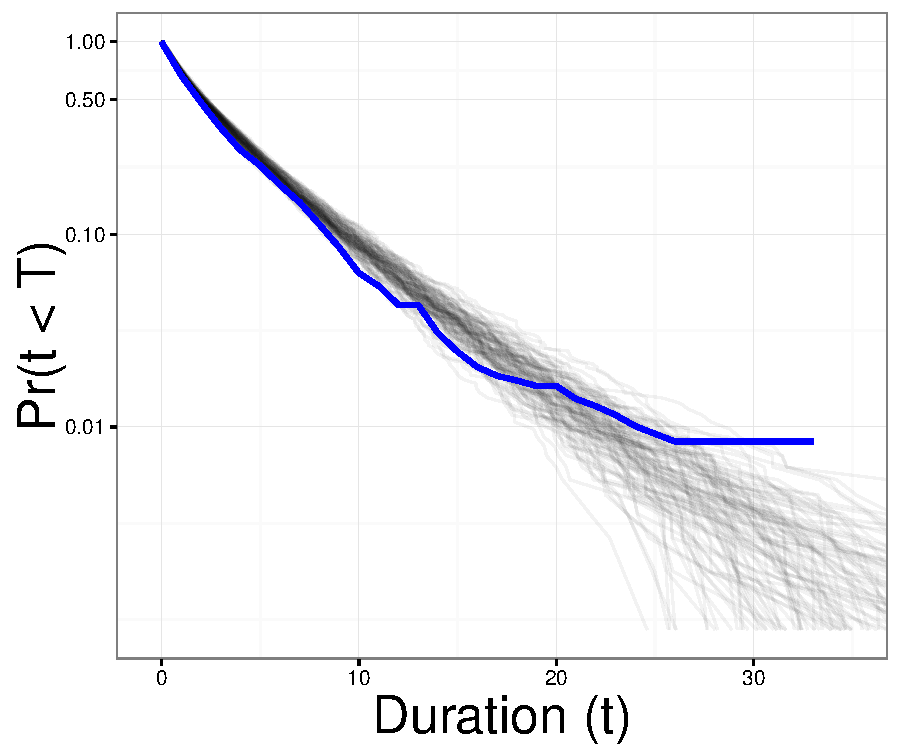
\includegraphics[height = 0.4\textheight,width=\textwidth,keepaspectratio=true]{chapter_preserve/figure/survival_curves}
  \caption[Posterior predictive check of survival]{Comparison of the empirical estimate of \(S(t)\) (highlighted) versus estimates from 100 posterior predictive data sets (black). \(S(t)\) corresponds to the probability that the age of a genus \(t\) is less than the genus' ultimate duration \(T\). The vertical axis is log10 transformed.}
  \label{fig:surv}
\end{figure}

\begin{figure}[ht]
  \centering
  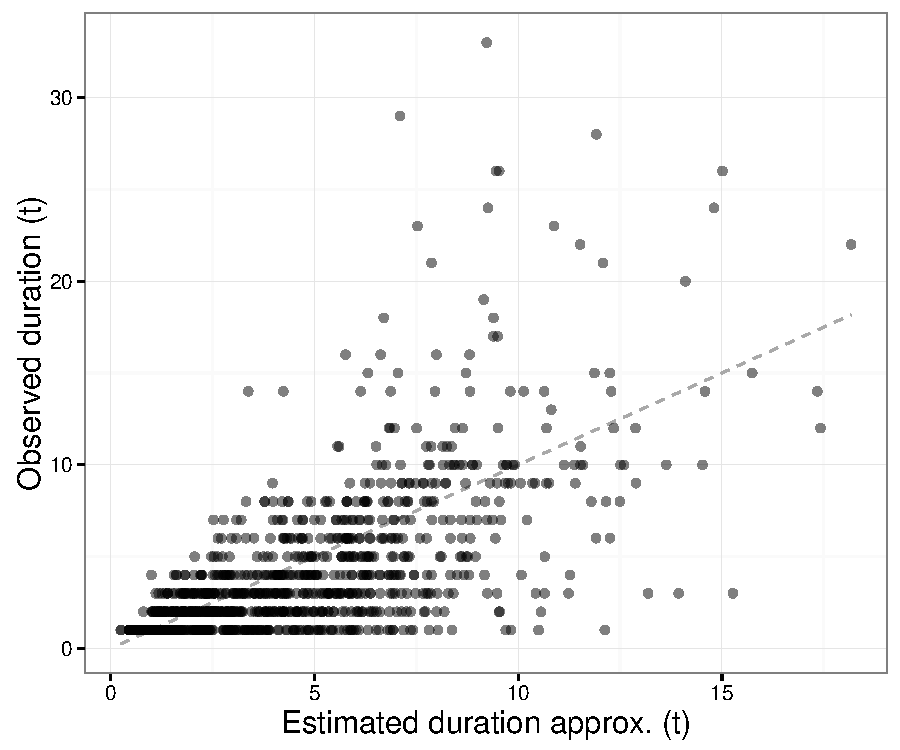
\includegraphics[height = 0.4\textheight,width=\textwidth,keepaspectratio=true]{chapter_preserve/figure/shotgun}
  \caption[Posterior predictive check of congruence]{Comparison of all observed genus durations in number of geological stages to the average posterior predictive estimates of \(\log(\sigma)\). The dashed, diagonal line corresponds to \(x = y\).}
  \label{fig:shot}
\end{figure}

The cohort-level estimate of the effect of geographic range size indicates that as a taxon's geographic range increases, that taxon's duration is expected to increase (Table \ref{tab:param}). Given the estimates of \(\mu^{r}\) and \(\tau^{r}\), there is a less than 3.7\% (\(\pm 0.04\%\) SD) probability that this relationships would be reversed (\(\mathrm{Pr}\mathcal{N}(\mu^{r}, \tau^{r}) > 0)\)). The between-cohort variance \(\tau^{r}\) is the lowest of all the regression coefficients (Table \ref{tab:param}).

Body size is estimated to have no effect on taxon duration, with the estimate being nearly 0 (Table \ref{tab:param}). The variance between the cohort-specific estimates of the effect of body size \(\tau^{m}\) is estimated to be greater than the variance of between-cohort estimates of the effect of geographic range size \(\tau^{r}\). 

The group-level estimate of the effect of environmental preference is estimated from both \(\mu^{v}\) and \(\mu^{v^{2}}\). 

The estimate of \(\mu^{v}\) indicates that epicontinental favoring taxa are expected to have a greater duration than open-ocean favoring taxa (Table \ref{tab:param}). Additionally, given the estimate of between-cohort variance \(\tau^{v}\), there is approximately 18\% (\(\pm 7\%\) SD) probability that, for any given cohort, taxa favoring open-ocean environments would have a greater expected duration than taxa favoring epicontinental environments (\(\mathrm{Pr}(\mathcal{N}(\mu^{v}, \tau^{v}) > 0)\)). 

The estimate of \(\mu^{v^{2}}\) indicates that the overall relationship between environmental preference and \(\log(\sigma)\) is concave down (Fig. \ref{fig:env_mean}), with only a 2.7\% (\(\pm 3\%\) SD) probability that any given cohort is convex up (\(\mathrm{Pr}(\mathcal{N}(\mu^{v^{2}}, \tau^{v^{2}}) < 0\)).

\begin{figure}[ht]
  \centering
  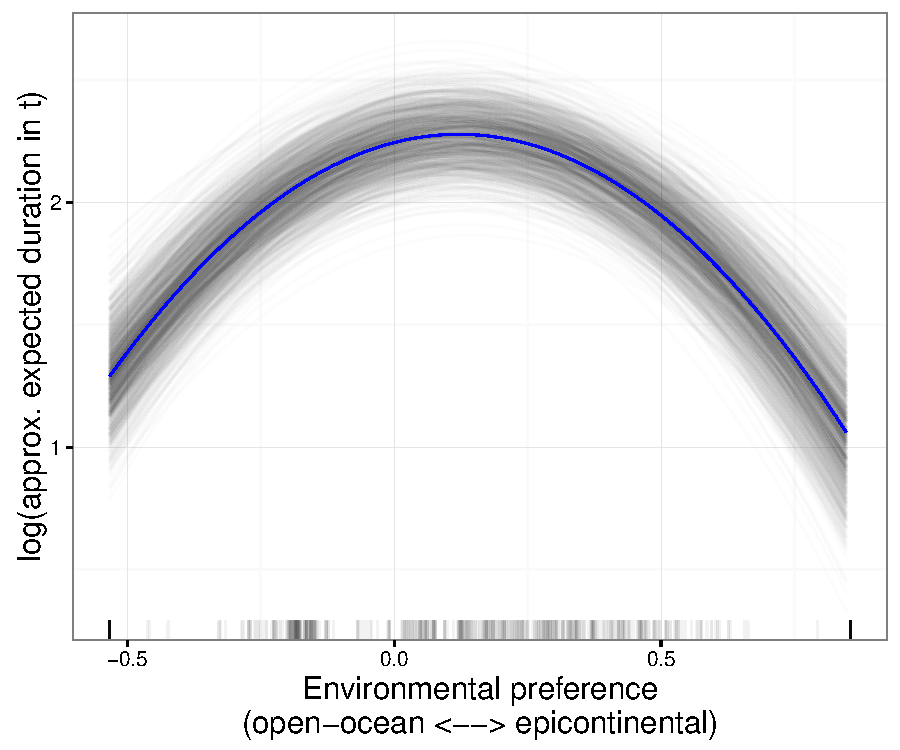
\includegraphics[height = 0.4\textheight,width=\textwidth,keepaspectratio=true]{chapter_preserve/figure/env_effect}
  \caption[Estimated relationship between environment and survival]{The overall expected relationship between environmental affinity \(v_{i}\) and a \(\log(\sigma)\) when r = 0 and m = 0. The 1000 semi-transparent lines corresponds to a single draw from the posterior predictive distribution, while the highlighted line corresponds to the median of the posterior predictive distribution. The overall relationship is concave down with an optimum greater than 0, which means that taxa favoring epicontinental environments are expected to have longer durations than those favoring open-ocean environments. The tick marks along the bottom of the plot correspond to the (rescaled) observed values of environmental preference.}
  \label{fig:env_mean}
\end{figure}


\afterpage{\clearpage}
\begin{figure}[p]
  \centering
  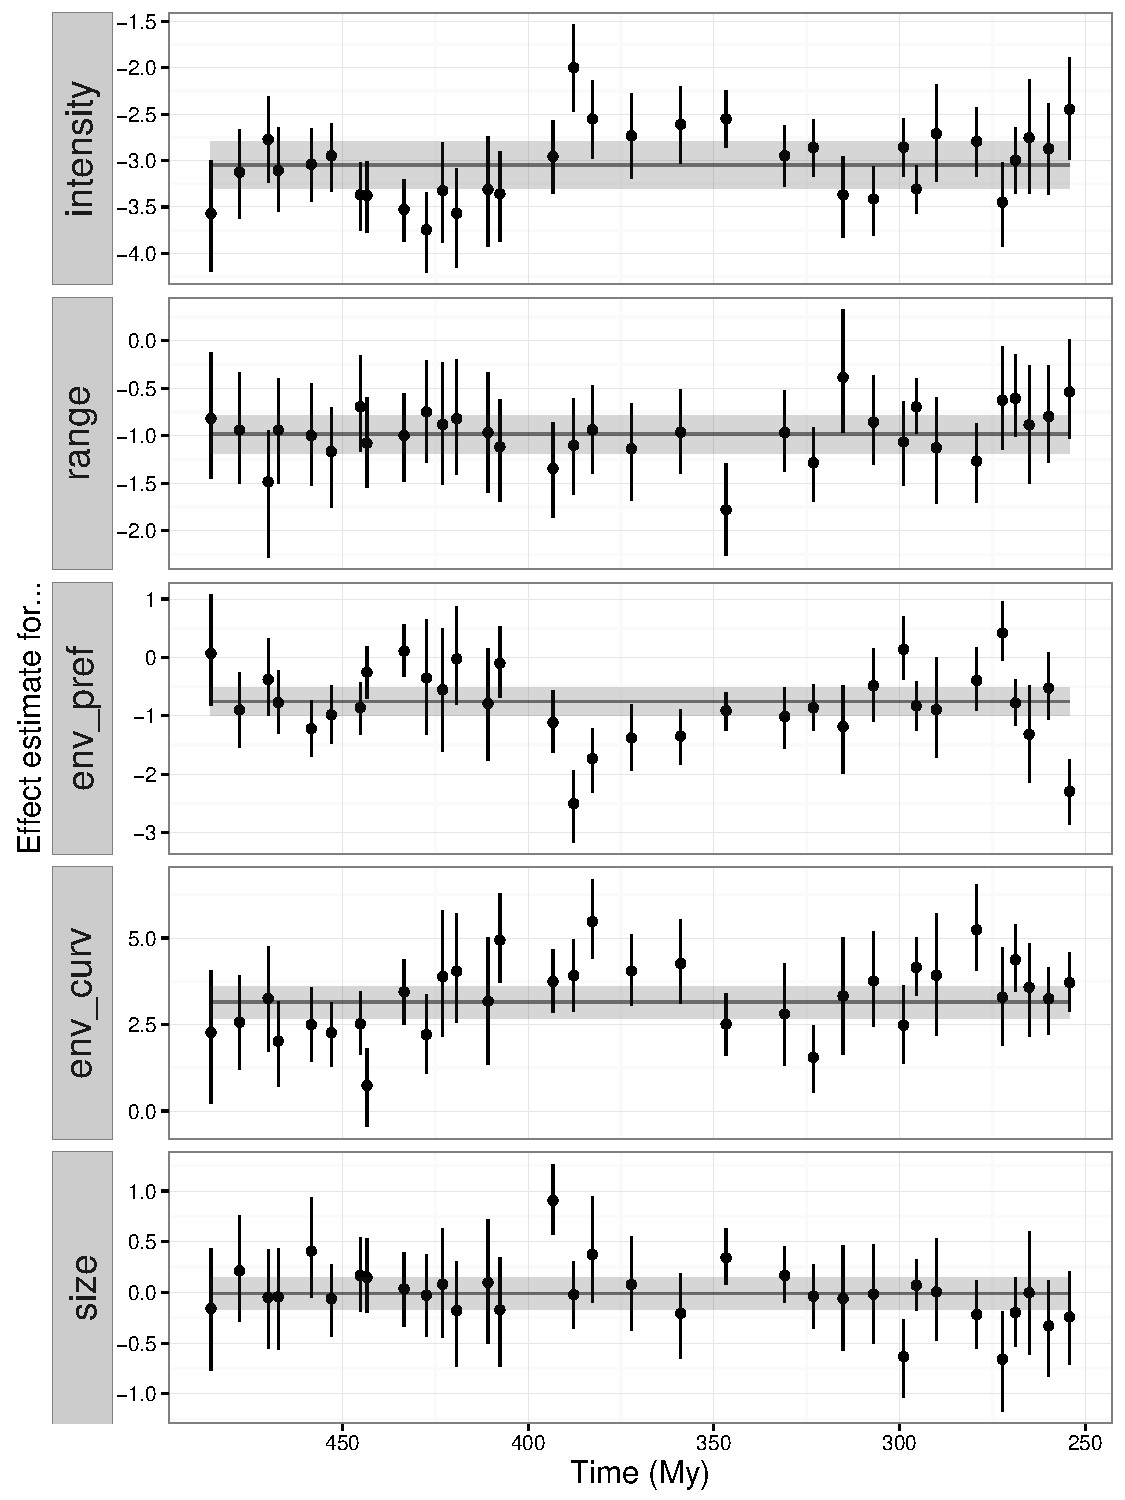
\includegraphics[width = \textwidth,height = 0.8\textheight,keepaspectratio=true]{chapter_preserve/figure/cohort_series}
  \caption[Cohort specific relationship between environment and survival]{Comparison of cohort-specific estimates of \(\beta^{0}\), the effect of geographic range on extinction risk \(\beta^{r}\), the effect of environmental preference \(\beta^{v}\) and \(\beta^{v^{2}}\), and body size \(\beta^{m}\). Points correspond to the median of the cohort-specific estimate, along with 80\% credible intervals. Points are plotted at the midpoint of the cohorts stage of origination in millions of years before present (My). Black, horizontal lines are the overall estimates of covariate effects along with 80\% credible intervals (shaded).}
  \label{fig:cohort_series}
\end{figure}

The cohort-specific estimates of all the regression coefficients demonstrate a lot of between cohort variance, with no obvious trends. As indicated in Table \ref{tab:param} and detectable visually (Fig. \ref{fig:cohort_series}), the between-cohort estimates for \(\beta^{0}\), \(\beta^{r}\), and \(\beta^{m}\) all have much lower variance than the between-cohort estimates of both \(\beta^{v}\) and \(\beta^{v^{2}}\).

While most cohort-specific estimates are very similar to the overall cohort-level estimate, there are a few notable excursions away from the overall mean (Fig. \ref{fig:cohort_series}). There are simultaneous excursions in both \(\beta^{0}\) and \(\beta^{v}\) for cohorts originating in the Givetian (387-382 My) and Frasnian (382-372 My) stages; both of which directly precede the late Devonian mass extinction event at the Frasnian/Famennian boundary. These cohorts are marked by both a high extinction intensity and an increase in expected duration for taxa favoring epicontinental environments over open-ocean ones.%; this is consistent with the results of Miller and Foote \citep{Miller2009a}.

Cohorts originating from the Silurian through the Early Devonian have a slightly lower extinction intensity than the overall mean; these cohorts are those originating in the Llandovery (443-443 My) through the Emsian (407-393 My). These time periods are when there is the lowest overall probability that epicontinental favoring taxa are expected to have greater duration than open-ocean favoring taxa. Both the Silurian and Devonian periods are notable for having been periods with a mostly ``hothouse'' climate, with no polar icecaps and a high sea-level \citep{Edwards1985,Joachimski2009,Munnecke2010}.
% Probability inflection point > 0 for cohorts 6 (Kantian) through 15 (Eifelian):
%   0.99, 0.99, 0.632, 0.377, 0.685, 0.754, 0.52, 0.851, 0.581, 0.995

% cohort-specific environmental effect
%   description of the variation in estimates
%   mass extinction boundaries
The cohort-specific relationships between environmental preference and \(\log(\sigma)\) were calculated from the estimates of \(\beta^{0}\), \(\beta^{v}\), and \(\beta^{v^{2}}\) (Fig. \ref{fig:env_cohort}) and reflect how these three parameters act in concert and not just individually (Fig. \ref{fig:cohort_series}). Beyond results already discussed above in the context of the parameters individually, it is notable that the cohort originating in the Kungurian (279-272 My) is least like the overall expected relationship and has the most sharply curved appearance due to a high estimate \(\beta^{v^{2}}\) (Fig. \ref{fig:cohort_series}). This cohort has the biggest difference in extinction risk between environmental generalists and specialists. The cohorts originating during the Emsian (407-393 My) and Frasnian (382 - 372 My) are tied for second in sharpness of curvature. The least sharply curved cohorts include those originating during Tremadocian (484-477 My), Hirnantian (445-443 My), Llandovery (443-433 My), and Ludlow (427-423 My). Except for the Tremadocian cohort, most of these cohorts originate during the Silurian through the Early Devonian range identified earlier as having lower expected extinction intensity than what is expected from the group-level estimate.

The correlations of the cohort-specific estimates of the regression coefficients are estimated as the off-diagonal elements of the correlation matrix \(\Omega\). Only two of the elements of \(\Omega\) are distinguishable from 0: the correlation of \(\beta^{0}\) (extinction intensity) with both \(\beta^{r}\) and \(\beta^{v}\) (Fig. \ref{fig:cor_posterior}). 

\afterpage{\clearpage}
\begin{figure}[p]
  \centering
  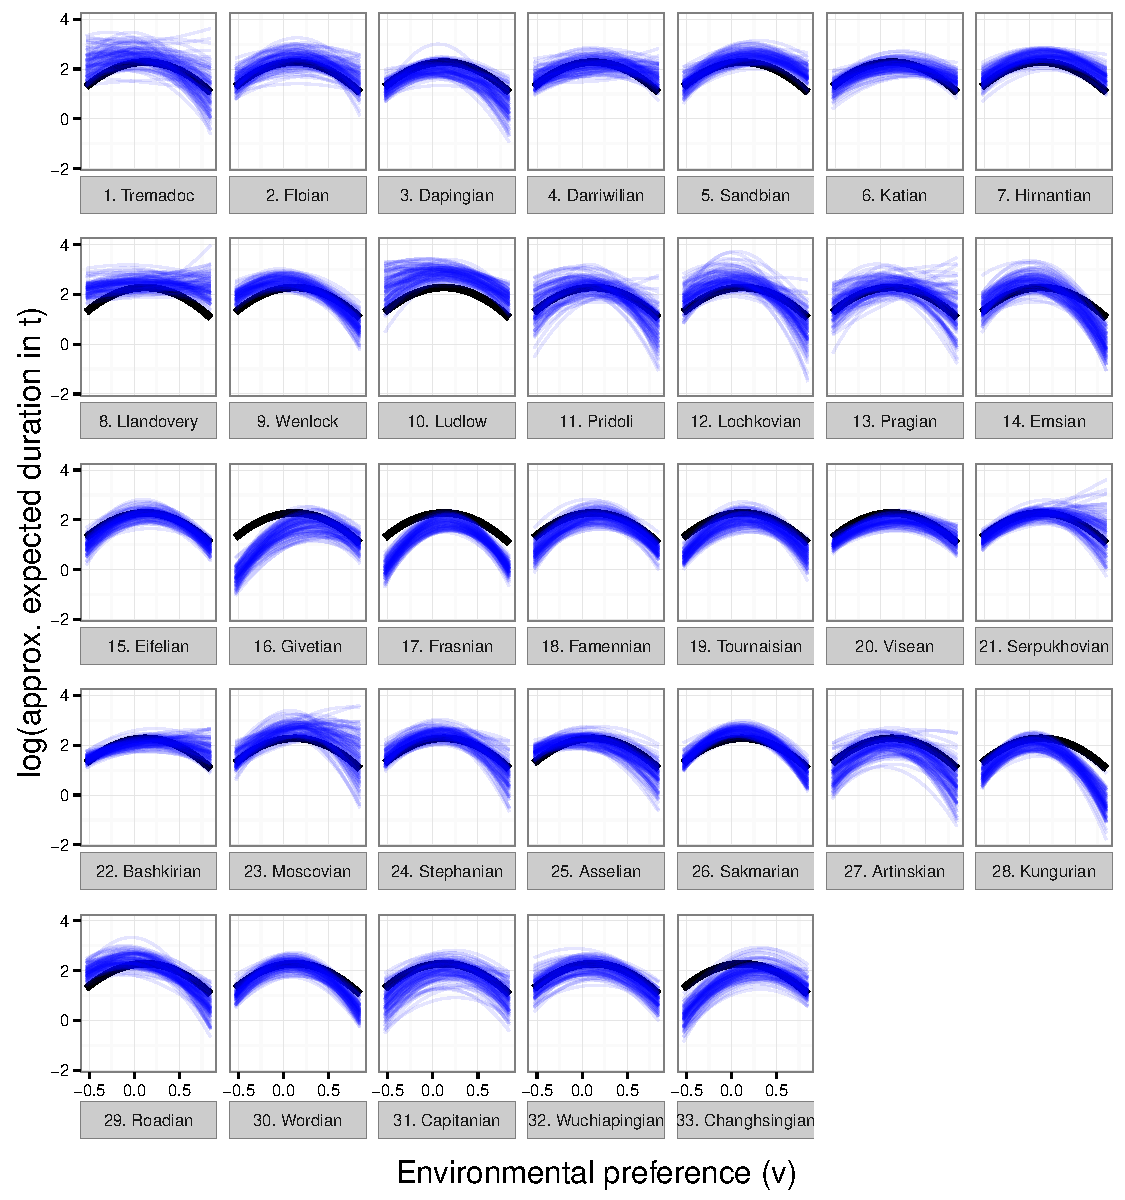
\includegraphics[width = \textwidth,height = 0.8\textheight,keepaspectratio=true]{chapter_preserve/figure/env_cohort}
  \caption[Effect of environmental covariates on survival]{Comparison of origination cohort-specific (posterior predictive) estimates of the effect of environmental preference on \(\log(\sigma)\) to the mean overall estimate of the effect of environmental preference. Cohort-specific estimates are from 100 posterior predictive simulations across the range of (transformed and rescaled) observed values of environmental preference. The oldest cohort is in the top-right and younger cohorts proceed left to right, with the youngest cohort being the right-most facet of the last row. Panel names correspond to the name of the stage in which that cohort originated.}
  \label{fig:env_cohort}
\end{figure}

\afterpage{\clearpage}
\begin{figure}[p]
  \centering
  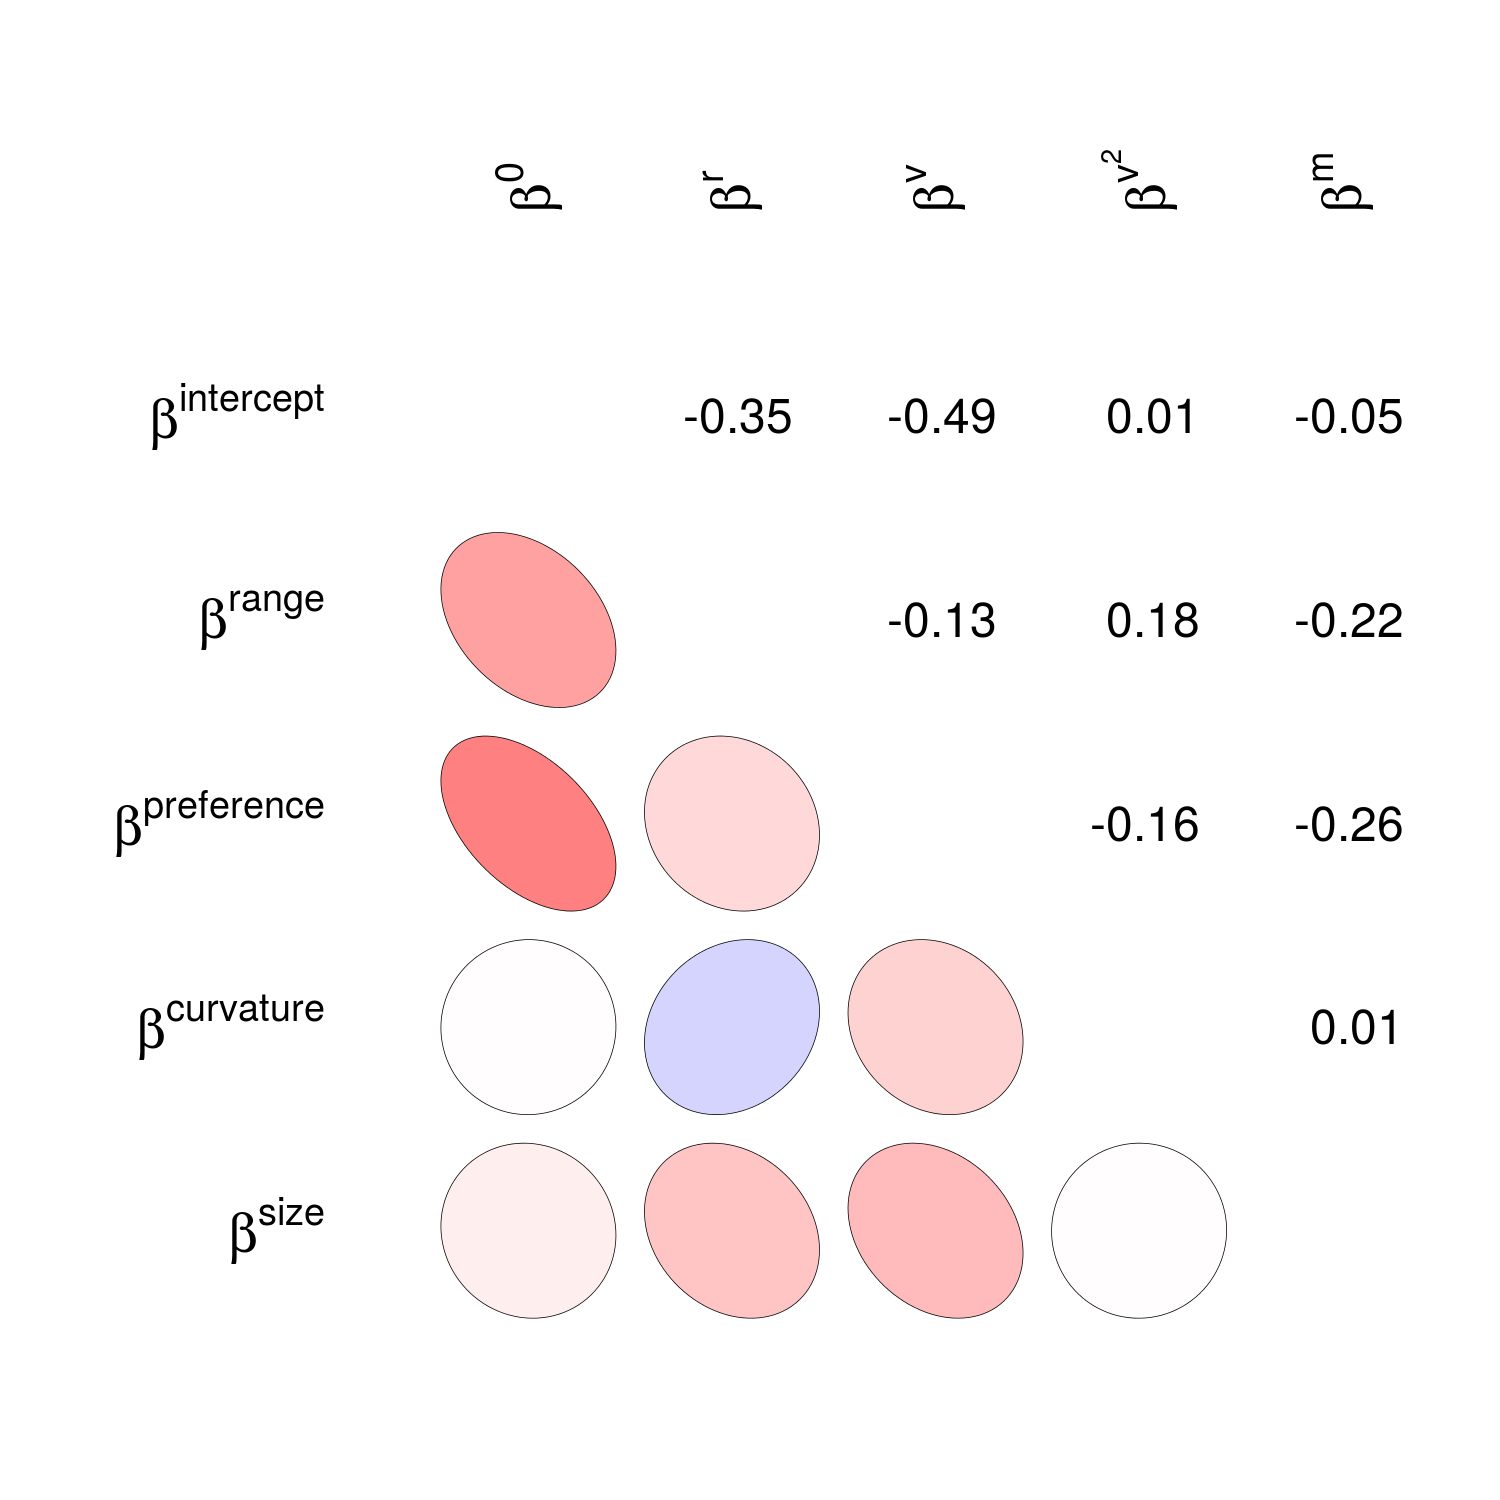
\includegraphics[height = 0.8\textheight,width=\textwidth,keepaspectratio=true]{chapter_preserve/figure/wei_cor_heatmap}
  \caption[Correlation matrix of effects of environmental covariates]{Mixed graphical and numerical representation of the correlation matrix \(\Omega\) of variation in cohort-specific covariate estimates. These correlations are between the estimates of the cohort-level effects of covariates, along with intercept/baseline extinction risk. The median estimates of the correlations are presented numerically (upper-triangle) and as idealized ellipses representing that much correlation (lower-triangle). The darkness of the ellipse corresponds to the magnitude of the correlation.}
  \label{fig:cor_posterior}
\end{figure}


There is an approximate 90\% probability that the cohort-specific estimates of baseline extinction intensity \(\beta^{0}\) and the effect of geographic range \(\beta^{r}\) are negatively correlated; this means that for cohorts experiencing a lower extinction intensity (\(\beta^{0}\) decreases), the magnitude of the effect of geographic range is expected to decrease as well, and \textit{vice versa}; this is in contrast to the observation made by Jablonski \citep{Jablonski1986} with regards to late Cretaceous bivalves.

Similarly, there is an approximate 97.4\% probability that the cohort-specific estimates of \(\beta^{0}\) and \(\beta^{v}\) are negatively correlated; this means that as extinction intensity increases it is expected that epicontinental taxa become more favored over open-ocean environments (i.e. as \(\beta^{0}\) increases, \(\beta^{v}\) decreases). 

There is only an approximate 30\% probability that \(\beta^{r}\) and \(\beta^{v}\) are positively correlated. This lack of cross-correlation may be due in part to the much higher between-cohort variance of the effect of environmental preference \(\tau^{v}\) than the very small between-cohort variance in the effect of geographic range \(\tau^{r}\) (Table \ref{tab:param}); the effect of geographic range might simply not vary enough relative to the much noisier environmental preference.

Comparison of observed values of sampling, as measured by the gap statistic, to random draws from the posterior estimates of the imputed sampling values indicate that they are very similar (Fig. \ref{fig:impute_results}. This result is very encouraging as this is the ultimate goal of multiple imputation: to fill in missing data with values similar to the observed while taking into account the randomness of that variable \citep{Rubin1996,Gelman2007}. The estimates of \(\delta\) are based on the set of observed values and the entire posterior of imputed values.

\begin{figure}[ht]
  \centering
  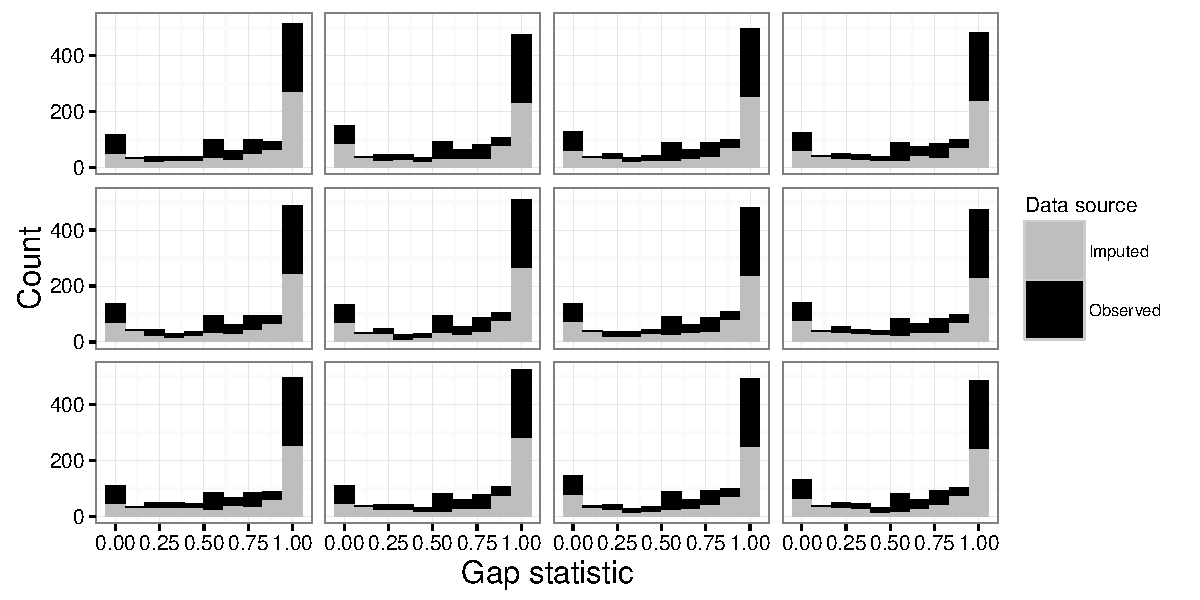
\includegraphics[height = 0.4\textheight,width=\textwidth,keepaspectratio=true]{chapter_preserve/figure/imputation_compare}
  \caption[Example imputed gap statistic distributions]{Histograms of the distribution of gap statistic values from both the observed values and the imputed values from 12 unique posterior realizations. For each panel the observed values are identical but the imputed values are from a single set of their posterior estimates.}
  \label{fig:impute_results}
\end{figure}

Sampling was found to have a negative effect (positive \(\delta\)) on duration: greater sampling, shorter duration (Table \ref{tab:param}). While potentially counter intuitive, this result is most likely due to some long lived taxa only be sampled in the stages of the first and last appearance. Also, longer lived taxa have more opportunities to not be sampled than shorter lived taxa. These two factors will lead to this result. 

While the effect of sampling appears large compared to the other regression coefficients, this is only because sampling was not standardized like the other covariates. To make the coefficients comparable, \(\delta\) is multiplied by twice the posterior mean of the standard deviation of sampling probability; the transformed value of \(\delta\) is then 0.642 (\(\pm 0.1\) SD). This effect is relatively small compared to the other covariate effects (Table \ref{tab:param}). There is then a 98.6\% probability that the effect of geographic range \(\mu^{r}\) has a greater magnitude than \(\delta\). Similarly, \(\mu^{v}\) has a 71.8\% probability of having a greater magnitude of effect than \(\delta\). Finally, \(\mu^{v^{2}}\) has a 100\% probability of having a greater magnitude of effect than \(\delta\).

The Weibull shape parameter \(\alpha\) was found to be approximately 1.36 (\(\pm 0.05\) SD) with a 100\% probability of being greater than 1. This result is not consistent with the Law of Constant Extinction \citep{VanValen1973} and is instead consistent with accelerating extinction risk with taxon age. This may indicate that older taxa are out-competed by younger taxa, a result consistent with some empirical results \citep{Wagner2014b,Quental2013,Smits2015b} and (ironically) with a recently proposed Red Queen-like model of evolution \citep{Rosindell2015a}. This results, however, is not consistent with other empirical results \citep{Finnegan2008,Crampton2016} and could potentially be caused by the minimum resolution of the fossil record \citep{Sepkoski1975}. It is thus unclear if a strong biological inference can be made from this result, which means that further work is necessary on the effect of taxon age on extinction risk.


\section{Discussion}

The generating observation behind this study was that for bivalves at the end Cretaceous mass extinction event, the only biological trait that was found to effect extinction risk was geographic range while traits that had previously been beneficial had no effect \citep{Jablonski1986}. This observation raises two linked questions: how does the effect of geographic range change with changing extinction intensity, and how does the effect of other biological traits change with changing extinction intensity?

I find that as intensity increases (\(\beta^{0}\) decreases), the magnitude of the effect of geographic range increases. I also find that as intensity increases, the effect of favoring epicontinental environments of open-ocean environments is expected to be increase; this is consistent with the results obtained by Miller and Foote \citep{Miller2009a}. There is no evidence for a correlation between the effect of geographic range and environmental preference. Additionally, the between-cohort variance in effect of geographic range is much less then the between-cohort variance of the effect of environmental preference which may underlie the lack of correlation between these two effects.

Additionally, the lower between-cohort variance in the effect of geographic range versus that higher between-cohort variance implies that for cohorts with a greater than average extinction intensity, the difference in the effect geographic range and the group-level effect of geographic range is expected to be smaller than the difference between the effect of environmental preference and the group-level effect of environmental preference.

I find consistent support for the ``survival of the unspecialized,'' with respect to epicontinental versus open-ocean environmental preference, as a time-invariant generalization of brachiopod survival; taxa with intermediate environmental preferences are expected to have lower extinction risk than taxa specializing in either epicontinental or open-ocean environments (Fig. \ref{fig:env_mean}), though the curvature of the relationship varies from rather shallow to very peaked (Fig. \ref{fig:env_cohort}). However, this relationship is not symmetric about 0, as taxa favoring epicontinental environments are expected to have a greater duration than taxa favoring open-ocean environments. This description of environment only describes one major aspect of a taxon's environmental context, with factors such as bathymetry and temperature being further descriptors of a taxon's adaptive zone \citep{Nurnberg2013a,Harnik2013,Harnik2011,Heim2011}; inclusion of these factors in future analyses would potentially improve our understanding of the ``survival of the unspecialized'' hypothesis \citep{Simpson1944}.

Hopkins \textit{et al.} \citep{Hopkins2014a}, in their analysis of niche conservatism and substrate lithological preference in marine invertebrates, found that brachiopods were among the least ``conservative'' groups; taxa were found to easily change substrate preference on short time scales. While substrate preference is not the same as environmental preference (as defined here), a question does arise: are there three classes of environmental preference instead of two? These classes would be taxa with broad tolerance (``true'' generalists), inflexible specialists (``true'' specialists), and flexible but with a narrow tolerance. A flexible taxon is one with a narrow habitat preference at one time, but with preference that changes over time with changing environmental availability. My analysis assumes that traits are constant over the duration of the taxon meaning that this scenario is not detectable; taxa with broad tolerances and flexible taxa with narrow per-stage preference end up being treated the same way. Future work should explore how environmental preference changes over lineage duration in relation to environmental availability to estimate if the generalists--specialists continuum is actually ternary relationship.

An alternative approach for specifically modeling survival that can take into account imperfect observation than the method used here is the Cormack-Jolly-Seber (CJS) model \citep{Royle2008,Liow2008,Tomiya2013,Liow2010b}. This model is a type of hidden Markov model with an absorbing state (i.e. extinction). In this model, survival is defined as the probability of surviving from time \(t\) to time \(t + 1\). Additionally, the effect of preservation and sighting is estimated as probability of observing a taxon that is present; this can extend the duration of a taxon beyond its last occurrence. This approach is a fundamentally different from the method used in my analysis: I am estimating the biasing effect of sampling probability on taxon duration to then compare with effects of other covariates, while the CJS model estimates the pre-sampling fossil record and then estimates per-time unit survival probability.

% discussion of context of study
%   defense
%     species:genus?
%     difficulty towards tails, but that's to be expected
%       this model is about expectations, not tails/extreme events
%       this model is ok for the main part of the data
%       though, of course, this model has a long way to go (all models are false)
The use of genera as the unit of the study and how to exactly interpret the effects of the biological traits is an important question. For example, if any of the traits analyzed here are associated with increases in speciation rates, this might increase the duration of genera through self-renewal \citep{Raup1991b,Raup1994}, which would be an example of the difference in biological pattern between species and genera \citep{Jablonski1987,Jablonski2007,Jablonski2008a}. This could lead to a trait appearing to decrease generic level extinction risk by that trait increasing species level origination rate instead of decreasing species level extinction risk. % conflict between levels in effect: genus duration increased by speciation, not extinction of species

% future direction
The model used here could be improved through either increasing the number of analyzed traits, expanding the hierarchical structure of the model to include other major taxonomic groups of interest, and the inclusion of explicit phylogenetic relationships between the taxa in the model as an additional hierarchical effect. An example trait that may be of particular interest is the affixing strategy or method of interaction with the substrate of the taxon, which has been found to be related to brachiopod survival where, for cosmopolitan taxa, taxa that are attached to the substrate are expected to have a greater duration than those that are not \citep{Alexander1977}.

%   comparison with other major groups in hierarchical model
It is theoretically possible to expand this model to allow for comparisons both within and between major taxonomic groups which would better constrain the brachiopod estimates while also allowing for estimation of similarities and differences in cross-taxonomic patterns. The major issue surrounding this particular expansion involves finding a similarly well sampled taxonomic group that is present during the Paleozoic. Potential groups include Crinoidea, Ostracoda, and other members of the ``Paleozoic fauna'' \citep{Sepkoski1981a}.

With significant updates, it would also be possible to compare the brachiopod record with with Moden groups such as bivalves or gastropods \citep{Sepkoski1981a}, though remembering that the groups may not necessarily share all cohorts with the brachiopods. This particular model expansion would act as a test of any universal cross-taxonomic patterns in the effects of emergent traits on extinction such as has been proposed for geographic range \citep{Payne2007}. Additionally, this expanded model would also act as a test of the distinctness of the Sepkoski's three-fauna hypothesis \citep{Sepkoski1981a} in terms of trait-dependent extinction.

Traits like environmental preference or geographic range \citep{Jablonski1987,Hunt2005a} are most likely heritable. Without phylogenetic context, this analysis assumes that differences in extinction risk between taxa are independent of the shared evolutionary history of those  taxa \citep{Felsenstein1985b}. In contrast, the origination cohorts only capture shared temporal context. For example, if taxon duration is phylogenetically heritable, then closely related taxa may have more similar durations as well as more similar biological traits. Without taking into account phylogenetic similarity the effects of these biological traits would be inflated solely due to inheritance. The inclusion of phylogenetic context as an additional individual-level hierarchical effect, independent of origination cohort, would allow for determining how much of the observed variability is due to shared evolutionary history versus shared temporal context versus actual differences associated with biological traits \citep{Smits2015b}.

The combination and integration of the phylogenetic comparative and paleontological approaches requires both sources of data, something which is not possible for this analysis because there is no phylogenetic hypothesis for all Paleozoic taxa, something that is frequently the case for marine invertebrates with a good fossil record. When both data sources are available has been possible, however, the analysis can more fully address the questions of interest in macroevolution \citep{Smits2015b,Slater2013a,Slater2015c,Simpson2011,Tomiya2013,Slater2012,Raia2013c,Raia2012f,Harnik2014,Fritz2013a}.

% concluding statements
In summary, patterns of Paleozoic brachiopod survival were analyzed using a fully Bayesian hierarchical survival modelling approach while also eschewing the traditional separation between background and mass extinction. I find that cohort extinction intensity is negatively correlated with both the cohort-specific effects of geographic range and environmental preference. These results imply that as extinction intensity increases (\(\beta^{0}\)) it is expected that both effects will increase in magnitude. However, the change in effect of environmental preference is expected to be greater than the change in the effect of geographic range. Additionally, I find support for greater survival in environmental generalists over specialists in all origination cohorts analyzed; this is consistent with the long standing ``survival of the unspecialized'' hypothesis \citep{Liow2004a,Liow2007b,Simpson1944,Simpson1953,Smits2015b,Nurnberg2015,Nurnberg2013a, Baumiller1993}. The results of this analysis support the conclusion that for Paleozoic brachiopods, as extinction intensity increases overall extinction selectivity is expected to increase as well.


%\section*{Acknowledgements}
%I would like to thank K. Angielzcyk, M. Foote, P. D. Polly, R. Ree, and G. Slater for helpful discussion during the conception of this study. I'd also like to thank D. Bapst, N. Pierrehumbert and M. Villarosa Garcia for additional comments. An additional thank you to  A. Miller for the epicontinental versus open-ocean assignments. Finally, thank you to the reviewers for their helpful comments that improved this manuscript. This entire study would would not have been possible without the Herculean effort of the many contributors to the Paleobiology Database. In particular, I would like to thank J. Alroy, M. Aberhan, D. Bottjer, M. Clapham, F. F\"{u}rsich, N. Heim, A. Hendy, S. Holland, L. Ivany, W. Kiessling, B. Kr\"{o}ger, A. McGowan, T. Olszewski, P. Novack-Gottshall, M. Patzkowsky, M. Uhen, L. Villier, and P. Wager. This work was supported by a NASA Exobiology grant (NNX10AQ446) to A. Miller and M. Foote. I declare no conflicts of interest. This is Paleobiology Database publication XXX. The code necessary for reproducing these results is avaliable as a Zenodo archive DOI 10.5281/zenodo.46928.


%\clearpage
%
%
%\bibliographystyle{evolution}
%\bibliography{newbib,packages}
%
%
%\clearpage


%\begin{table}[h]
\begin{sidewaystable}
  \centering
  \caption[Parameter estimates for brachiopod survival model]{Estimates of various parameters in the model used here. These include group-level estimates of the effects of biological traits on brachiopod generic survival, the standard deviation of the between-cohort effects, as well as the estimates of both the effect of sampling \(\delta\) and the Weibull shape parameter \(\alpha\). The mean, standard deviation (SD), 10th, 50th, and 90th quantiles of the marginal posteriors are presented.}
  \begin{tabular}{ l | l p{2.5cm} r r r r r }
    \hline
    type & parameter & effect of & mean & SD & 10\% & 50\% & 90\% \\ 
    \hline
    \multirow{5}{*}{Mean} & \(\mu^{i}\) & intercept & -3.05 & 0.20 & -3.30 & -3.05 & -2.80 \\
    & \(\mu^{r}\) & geographic range & -0.98 & 0.16 & -1.18 & -0.98 & -0.79 \\
    & \(\mu^{v}\) & environmental preference & -0.76 & 0.19 & -0.99 & -0.76 & -0.52 \\
    & \(\mu^{v^{2}}\) & environmental preference\(^{2}\) & 3.15 & 0.36 & 2.69 & 3.15 & 3.62 \\
    & \(\mu^{m}\) & body size &  -0.01 & 0.13 & -0.17 & -0.01 & 0.15 \\
    \hline
    \multirow{5}{*}{Standard deviation} & \(\tau^{i}\) & intercept & 0.51 & 0.11 & 0.38 & 0.50 & 0.65 \\
    & \(\tau^{r}\) & geographic range & 0.50 & 0.16 & 0.30 & 0.49 & 0.71 \\ 
    & \(\tau^{v}\) & environmental preference & 0.84 & 0.17 & 0.63 & 0.82 & 1.05 \\
    & \(\tau^{v^{2}}\) & environmental preference\(^{2}\) & 1.51 & 0.36 & 1.08 & 1.48 & 1.97 \\
    & \(\tau^{m}\) & body size & 0.47 & 0.13 & 0.32 & 0.46 & 0.64 \\ 
    \hline
    \multirow{2}{*}{Other} & \(\delta\) & sampling & 0.90 & 0.15 & 0.71 & 0.90 & 1.09 \\ 
    & \(\alpha\) & ``time'' & 1.36 & 0.04 & 1.30 & 1.36 & 1.42 \\ 
    \hline
  \end{tabular}
  \label{tab:param}
%\end{table}
\end{sidewaystable}


% chapter 3
\chapter{Taxon occurrence as a function of both emergent biological traits and its environmental context}

Place holder text.


\chapter{Conclusion}

% Format a LaTeX bibliography
\makebibliography

% Figures and tables, if you decide to leave them to the end
%\input{figure}
%\input{table}

\end{document}
